 %Hauptdokumentation der Lösung
\NeedsTeXFormat{LaTeX2e}

\documentclass[a4paper,oneside,abstract]{scrreprt}
\usepackage{FHNW}
\usepackage{pdfpages}
\usepackage{comment}
\usepackage{framed}
\usepackage{paralist}
\usepackage{float}
\usepackage{setspace}
\pagestyle{fancy}
\usepackage[nottoc,numbib]{tocbibind}

\newcommand{\titel}{Detroit Electric Car}
\newcommand{\shorttitel}{Yanick Frei, Marc Müller}
\newcommand{\doctype}{Fachbericht Projekt 5 EIT}
\newcommand{\untertitel}{Umrüsten eines Detroit Electric Car von 1918 auf Li-Ion Batterien}
\newcommand{\datum}{\today}
\newcommand{\autorA}{Yanick Frei}
\newcommand{\autorB}{Marc Müller}
\newcommand{\ort}{Windisch}
\newcommand{\dozent}{Urs Jäger}
\newcommand{\betreuer}{Felix Jenni}
\newcommand{\version}{1.0}

\title{\titel}
\author{\autorA  \and \AutorB \and \AutorC \and \AutorD \and \AutorE}
\date{\datum}


\begin{document}


%%%%%%%%%%%%%%%%%%%%%%%%%%%%%%%%%%%%%%%%%%%%%%%%%%%%%%%%%%%%%%%%%%%%%%%%%%%%%%%%
% Titelseite
%%%%%%%%%%%%%%%%%%%%%%%%%%%%%%%%%%%%%%%%%%%%%%%%%%%%%%%%%%%%%%%%%%%%%%%%%%%%%%%%
% title page -------------------------------------------------------------------
\thispagestyle{plain}

\begin{titlepage}
	\begin{flushleft}
		\textbf{
			\hspace{-0.12cm}\LARGE{\doctype}\\
			\Huge{\titel}\\
			\vspace{0.5cm}
			\large{\untertitel}
		}
		\vspace{1cm}
		\vfill
		\large{
			\hspace{-1cm} 
\includegraphics{images/fhnw_logo_full}\\
			\line(1,0){165}	

			\vspace{0.5cm}
			\textbf{Autoren:}\\ \autorA\\ \autorB \\
			\vspace{0.5cm}
			\textbf{Auftraggeber:}\\ \dozent \\
			\vspace{0.5cm}
			\textbf{Fachcoach:}\\ \betreuer \\
			\vspace{0.5cm}
			\ort, \datum \hfill Version: \version
			\\
		}
	\end{flushleft}
\end{titlepage}
% end of titlepage -------------------------------------------------------------


%%%%%%%%%%%%%%%%%%%%%%%%%%%%%%%%%%%%%%%%%%%%%%%%%%%%%%%%%%%%%%%%%%%%%%%%%%%%%%%%
% Abstract
%%%%%%%%%%%%%%%%%%%%%%%%%%%%%%%%%%%%%%%%%%%%%%%%%%%%%%%%%%%%%%%%%%%%%%%%%%%%%%%%
\pagenumbering{gobble}
{\pagestyle{plain}{
	\setcounter{tocdepth}{2}
	\chapter*{Abstract}


}}

\clearpage
\pagestyle{plain}
\pagenumbering{Roman}
\renewcommand{\chaptermark}[1]{\markboth{#1}{}}

%%%%%%%%%%%%%%%%%%%%%%%%%%%%%%%%%%%%%%%%%%%%%%%%%%%%%%%%%%%%%%%%%%%%%%%%%%%%%%%%
% Inhaltsverzeichnis
%%%%%%%%%%%%%%%%%%%%%%%%%%%%%%%%%%%%%%%%%%%%%%%%%%%%%%%%%%%%%%%%%%%%%%%%%%%%%%%%
{\pagestyle{plain}{
\setcounter{tocdepth}{2}
\tableofcontents
}}

\clearpage
\fancyhdrplain
\pagestyle{plain}
\pagenumbering{arabic}
\renewcommand{\chaptermark}[1]{\markboth{#1}{}}

%%%%%%%%%%%%%%%%%%%%%%%%%%%%%%%%%%%%%%%%%%%%%%%%%%%%%%%%%%%%%%%%%%%%%%%%%%%%%%%%
% Einleitung
%%%%%%%%%%%%%%%%%%%%%%%%%%%%%%%%%%%%%%%%%%%%%%%%%%%%%%%%%%%%%%%%%%%%%%%%%%%%%%%%

\chapter{Einleitung}

Oldtimer sind begehrte Sammlerobjekte. Leider ist es aber auch die alte Technik, die diesen Fahrzeugen oft zum Verhängnis wird. So müssen Ersatzteile mit viel Handarbeit neu gemacht werden oder es müssen weitere Anpassungen gemacht werden, um den aktuellen Sicherheitsbestimmungen zu genügen. Ein anderer Ansatz ist deshalb, einen Teil der oftmals unsichtbaren Technik zu modernisieren und so die Probleme zu umgehen, was jedoch der historischen Korrektheit widerspricht.

Genau diese Vorgehensweise wurde beim vorliegenden Projekt gewählt: Ein beinahe einhundert jähriges Elektrofahrzeug soll auf moderne Lithium-Ionen-Akkumulatoren umgerüstet werden. Da das Fahrzeug, insbesondere die Batterie, bereits einmal umgebaut wurden, war diese nicht mehr von historischem Wert. Gleichzeitig sollte auch das sonstige Fahrzeug, insbesondere der elektrische Teil, begutachtet und gewartet werden, wobei die originale Schaltung beibehalten wird.

Die neue Batterie, die aus einem verunfallten Elektrofahrzeug stammt, musste auf das Fahrzeug angepasst werden, um an dessen Schaltung keine Anpassung vornehmen zu müssen. Auch das Batteriemanagementsystem zur Überwachung und Ausgleichung der Einzelzellen sowie das Ladegerät musste erneuert werden, da die Komponenten vom Unfallfahrzeug nicht übernommen werden konnten. Da solche Bauteile bereits existieren wurde auf eine Eigententwicklung verzichtet und auf käufliche Produkte zurück gegriffen.

Dieser Bericht beschränkt sich bewusst nicht nur auf die elektrotechnische Entwicklung. So sollen alle Komponenten, an denen gearbeitet wurde, erläutert werden, um so möglichst viele Informationen in diesem Bericht zu präsentieren. Diese Informationen sind dabei so gehalten, dass sie nicht nur von Ingenieuren, sondern auch von Laien verstanden werden können. Aus diesem Grund wurden auch immer wieder Erklärungen zu elektrotechnischen Vorgängen eingefügt, sodass die Arbeit mit möglichst wenig Vorkenntnissen verstanden werden kann.
\clearpage{\pagestyle{empty}\cleardoublepage}

\chapter{Der Detroit im Originalzustand}
In diesem ersten Kapitel soll der \textsc{Detroit}, wie er im Jahre 1918 war, vorgestellt werden. Dabei wird sowohl ein Blick auf die geschichtliche Entwicklung der Elektrofahrzeuge als auch auf den \textsc{Detroit} selbst geworfen. Von der Funktion des Detroits werden nur die Punkte erläutert, die sich im Vergleich zu heute geändert haben. Dies sind die Batterie und das zugehörige Ladegerät. Alle unveränderten Funktionen werden im Kapitel \ref{aktuell} "`Der Detroit im aktuellen Zustand"' vorgestellt.

\section{Geschichte}

Nachfolgend soll kurz die Firma \textsc{The Detroit Electric Car Company} vorgestellt werden. Im Anschluss wird spezifisch auf das Projektfahrzeug eingegangen.

\subsection{Firma}

Der \textsc{Detroit} aus dem Jahre 1918 ist bei weitem nicht der erste seiner Art. Seit dem Jahr 1907 fertigte die amerikanische Firma aus Detroit, welche bis dahin Pferdekutschen produzierte, Elektroautos. In den 1910er Jahren erreichten sie ihren Höhepunkt mit 1000 bis 2000 verkauften Autos pro Jahr. Mehrheitlich Frauen fuhren \textsc{Detroit}s, da sie sich zu schade für normale Autos waren. Diese Benzin- und Dieselfahrzeuge hatten damals noch keinen elektrischen Anlasser und somit musste der Motor mühsam per Hand angekurbelt werden. Auch waren damals Schadstofffilter noch unbekannt, womit sehr viele ungesunde Abgase in die Umwelt und die Gesichter der Damen geblasen wurde. Die Firma fabrizierte ihre Fahrzeuge bis in die späten 1930er Jahre. Danach wurden Elektroautos nicht weiter gefördert und die mächtige Ölindustrie unterstützte Fahrzeuge mit Verbrennungsmotoren. Somit war dies das Ende der Firma \textsc{Detroit Electric Car}.
In der heutigen Zeit ereignet sich mehrheitlich wieder ein Umdenken in den Köpfen der Menschen. Elektroautos sind umweltfreundlicher, günstiger im Unterhalt und modern, obwohl die Geschichte der Elektrofahrzeuge weiter zurückreicht als die der Benzinfahrzeuge.

\subsection{Der \textsc{Detroit} von 1918}
Beim Projektfahrzeug handelt es sich um einen blauen \textsc{Detroit Electric Car} aus dem Jahre 1918. Die korrekte Modellbezeichnung ist leider unbekannt, da es bei \textsc{Detroit} üblich war, die älteren Modelle zurückzukaufen und zu restaurieren. Weiter sind auch die früheren Besitzer dieses \textsc{Detroits} unbekannt. Es ist lediglich bekannt, dass unser Auftraggeber, Herr Jäger, das Fahrzeug von einem Bekannten gekauft hat. Vor diesem Kauf wurde das Fahrzeug in den USA restauriert. Jedoch stand das Fahrzeug über Jahre in einer Garage, da dieses nicht funktionierte und wurde erst anfangs 2017 an die FHNW Brugg-Windisch überführt, um die Fahrtüchtigkeit und die Umrüstung von Blei- auf Lithium-Ionen-Batterien sicherzustellen.
\section{Funktion der Bleibatterie}

Die Technik der Bleibatterien hat eine lange Geschichte welche bis in die Mitte des 19. Jahrhunderts zurückreicht. Diese sind heute in der Automobilindustrie eine schlechte und veraltete Alternative verglichen mit den modernen Lithium-Ionen-Akkumulatoren (siehe Kapitel \ref{kap_liion}). Zu dieser Zeit waren Bleibatterien jedoch die einzig sinnvolle Lösung Energie für den Eigengebrauch zu speichern. In diesem Kapitel soll die Grundfunktion einer Bleibatterie und die Lade-/Entladekurve erläutert werden.

\paragraph{Grundfunktion}
Grundsätzlich kommt die Bezeichnung Bleiakkumulator davon, dass beide Elektroden aus Blei, bzw. die positive Elektrode aus Bleidioxid (PbO$_2$) und die negative aus blankem Blei (Pb), besteht. Das Elektrolyt, was sich zwischen den Platten befindet, besteht aus Schwefelsäure (H$_2$SO$_4$). Im geladenen Zustand kann nun eine externe leitende Verbindung zwischen den beiden Elektroden gelegt werden. Dadurch zersetzt sich die positive Elektrode unter Elektronenabgabe, während die negative Elektrode Elektronen aufnimmt. Somit findet ein Ionenaustausch statt. Durch diesen Prozess wird der Akkumulator entladen und beide Elektroden bestehen nun aus Bleisulfat (PbSO$_4$). Der Ladeprozess funktioniert umgekehrt zum Entladeprozess. Durch Anlegen einer Spannung werden die Ionen wieder vom Minus- zum Plus-Pol transportiert. Auf weitere chemische Beschreibungen wird an dieser Stelle verzichtet. Der Lade- und Entladevorgang ist in Figur \ref{fig:pb_akku} ersichtlich \cite{pb_akku_funktion}:

\begin{figure}[h!]
	\centering
		\includegraphics[width=0.75\textwidth]{images/pb_akku.PNG}
	\caption{Lade-/Entladevorgang Blei-Akkumulator \cite{pb_akku_ent_lade}}
	\label{fig:pb_akku}
\end{figure}

\newpage

\paragraph{Lade-/Entladekurve}
Die Lade-/Entladekurve ist abhängig vom jeweiligen Akkumulatortyp. So auch die Bleibatterie, welche in Figur \ref{fig:pb_akku_kurve} für ein einzelnes Modul ersichtlich ist:

\begin{figure}[h!]
	\centering
		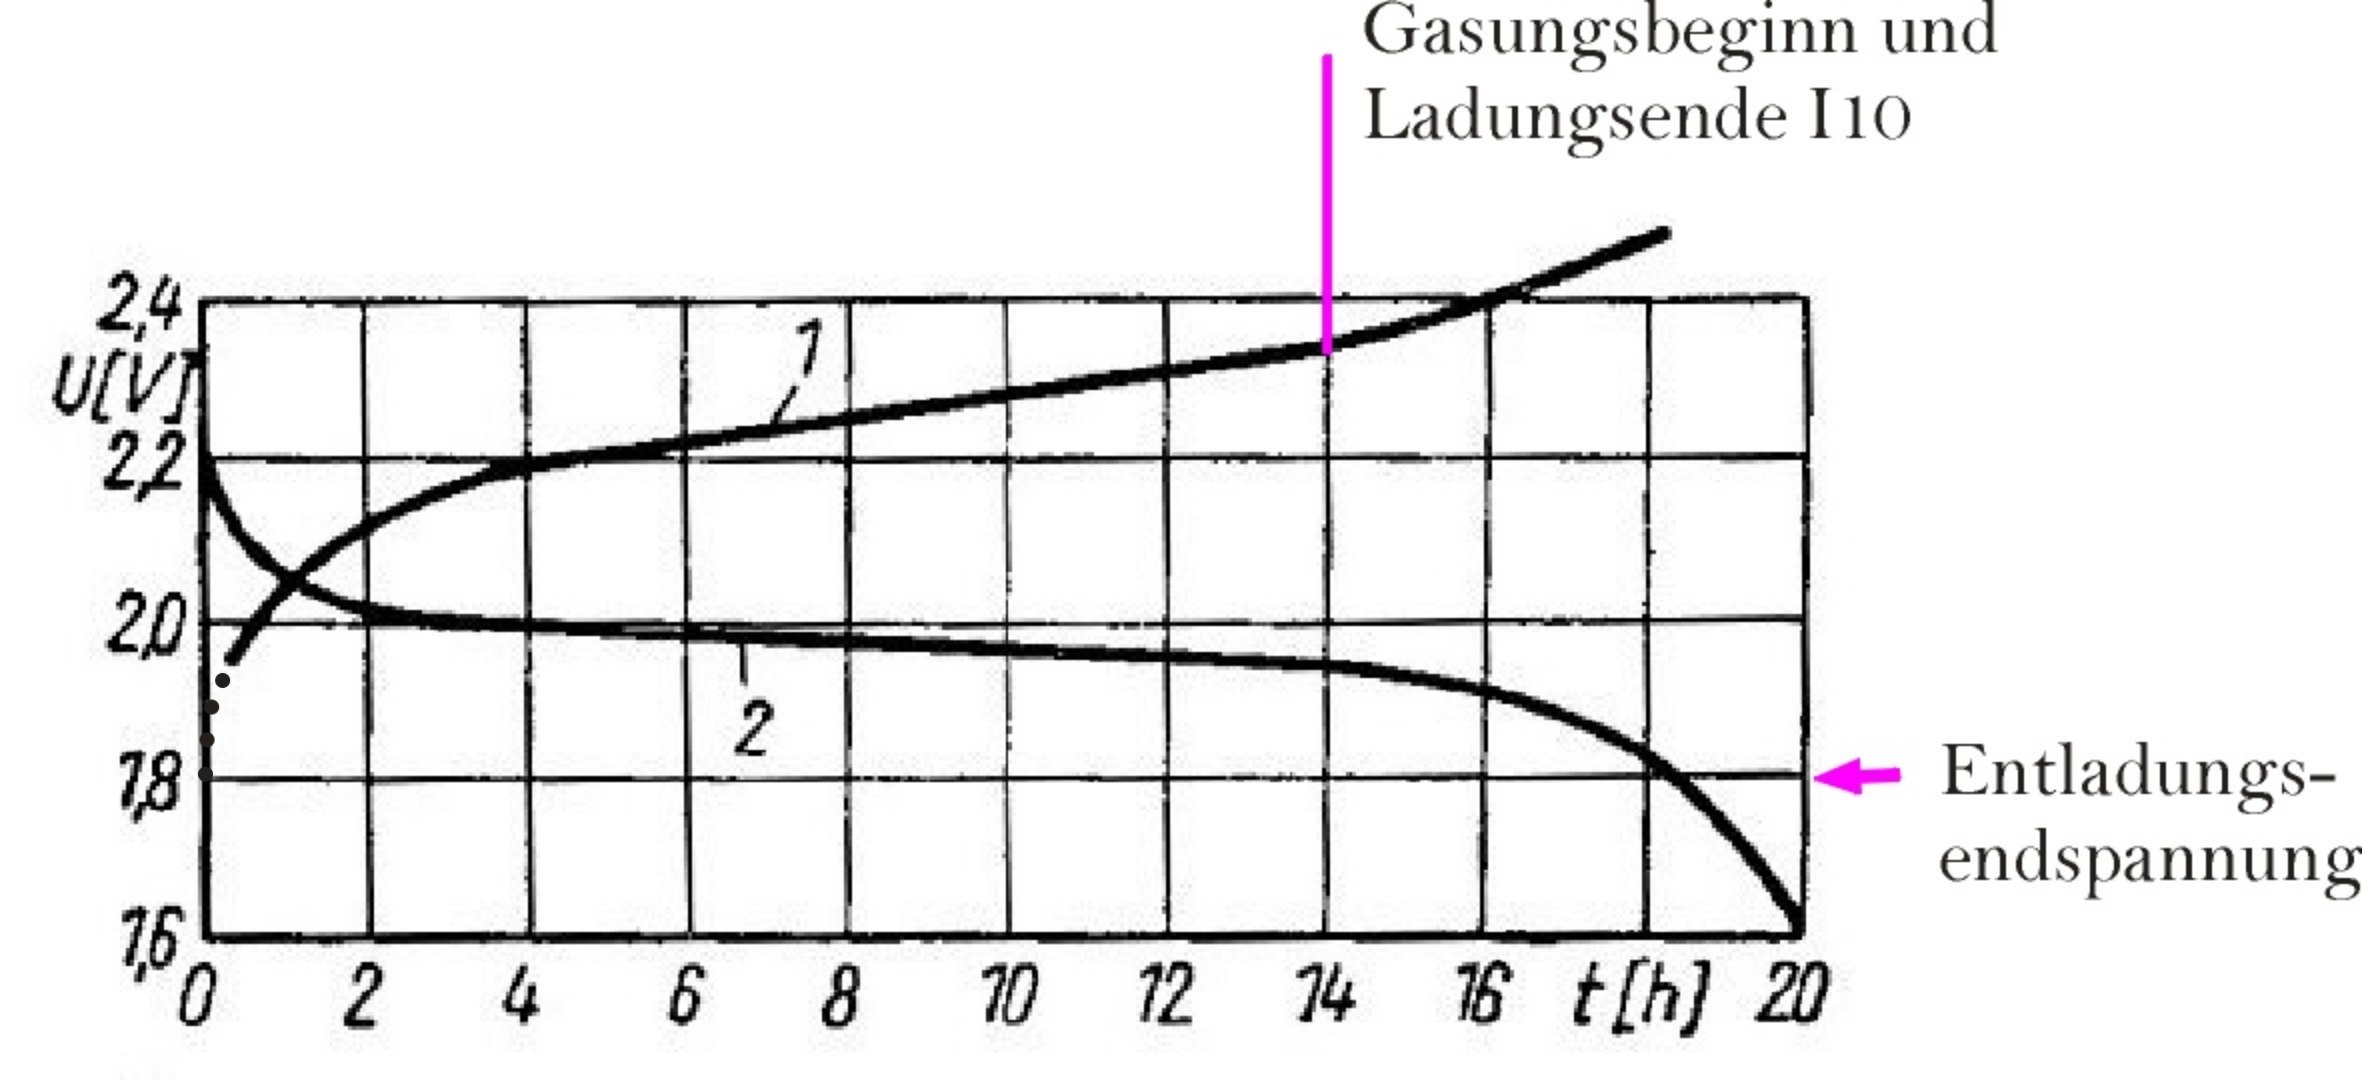
\includegraphics[width=0.8\textwidth]{images/pb_akku_kurve.jpg}
	\caption{Lade-/Entladekurve Blei-Akkumulator \cite{pb_akku_kurve}}
	\label{fig:pb_akku_kurve}
\end{figure}

In der obigen Figur kann man sehen, dass die Kurve im Zeitraum von 4 bis 14 Stunden einen konstante Anstieg im Ladevorgang oder Abstieg im Entladevorgang besitzt. Was unbedingt beachtet werden muss ist, dass ein einzelnes Bleimodul nicht unter $1.8$ V entladen oder über $2.3$ V geladen werden sollte. Dies könnte sonst zu einer Zerstörung des Moduls führen.

\newpage
\section{Originale Lademethoden}

Natürlich musste die Bleibatterie des \textsc{Detroit}s auch geladen werden. Für das Laden gab es zwei unterschiedliche Vorgehensweisen, die kurz vorgestellt werden sollen. Anschliessend wird auf das Ladegerät des \textsc{Detroit}s eingegangen.

\subsection{Laden in einer Garage} \label{Laden_in_Garage}
Viele Garagen boten an, das bei ihnen gekaufte Fahrzeug auch Laden zu lassen. So mussten die Garagen grosse Leistungen in Form von Gleichspannung zur Verfügung stellen. Diese Gleichspannung konnte auf zwei Arten erzeugt werden:

Ein \textbf{Umformer} ist eine Motor-Generator-Gruppe, die die Umformung von Wechsel- zu Gleichspannung über den Zwischenschritt der mechanischen Energie ermöglicht. Zu diesem Zweck wird ein erster Motor mit Wechselspannung gespeist. Auf der Achse dieses Motors sitzt eine weitere Maschine, die als Generator für Gleichspannung geschaltet ist. Wird diese Gleichspannungsmaschine als fremderregte Maschine ausgeführt, so ist die Spannung ausserdem in ihrem Betrag regelbar.

Alternativ kann die Gleichrichtung auch mit einer \textbf{Quecksilberdampfröhre} erfolgen. Dies ist eine Glasröhre, an deren unteren Ende sich flüssiges Quecksilber befindet, der als Kathode fungiert. Darüber befindet sich eine Heizwicklung, die zu Beginn das flüssige Quecksilber erwärmt und damit verdampfen lässt. Kondensiert dieses Quecksilber wieder, so kann es über die Glaswände zurück fliessen. Am oberen Ende der Glasröhre befindet sich eine Anode. Um das weitere Funktionsprinzip zu verstehen, muss ausserdem bekannt sein, dass sich die Elektronen sehr einfach aus dem Quecksilberdampf lösen können.

Nun sollen damit die beiden Spannungsrichtungen, die sich bei Wechselspannung mit der Netzfrequenz abwechseln, untersucht werden. Ist die Spannung von der Anode zur Kathode positiv, so werden die aus dem Quecksilberdampf gelösten Elektronen in Richtung der Anode beschleunigt und ein Stromfluss kommt zustande. Ist die Spannung zwischen Anode und Kathode hingegen negativ, so werden die gelösten Elektronen wieder zurück in den Quecksilbersee gezogen. Es fliesst also kein Strom zwischen Anode und Kathode. Da der Strom also nur während einer Spannungspolarität fliessen kann, steht am Ende eine \textcolor{blue}{pulsierende} Gleichspannung zur Verfügung.

Bei Privatfahrzeugen wurden die Batterien meist geladen, während sie sich im Auto befanden. Dazu wurden vom zentralen Gleichrichter Leitungen zu den einzelnen Ladestationen verlegt, bei welchen der Strom indirekt mittels eines stufenlosen Lastwiderstandes (eines sogenannten Rheostaten) reguliert werden konnte. Gerade bei Taxis oder Lastwagen war es aber auch weit verbreitet, die Batterien aus dem Fahrzeug zu entnehmen und in einem sogenannten "`Batterieraum"' zu laden. Das Fahrzeug konnte während dieser Zeit mit einem anderen Satz Batterien weiter benutzt werden. Beide Vorgehen sind in den Abbildungen \ref{fig:Laden_Garage} und \ref{fig:Laden_Batterieraum} auf der folgenden Seite gezeigt.

\begin{landscape}
\begin{figure}
\begin{minipage}{0.65\textwidth}
	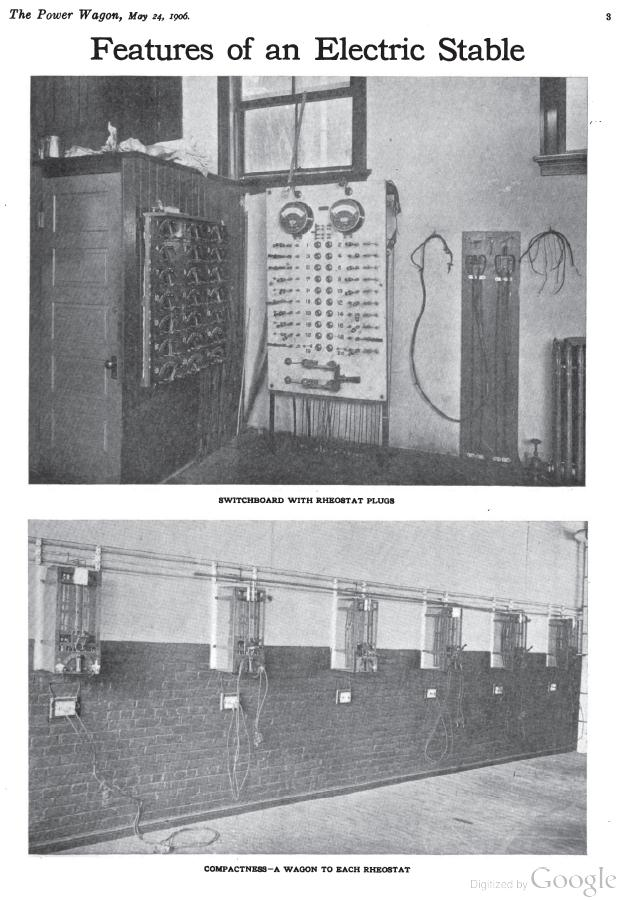
\includegraphics[width=\textwidth]{images/Laden_Garage.jpg}
	\caption{Ladestation für mehrere Fahrzeuge \cite{laden_alt}}
	\label{fig:Laden_Garage}
\end{minipage}
\begin{minipage}{0.65\textwidth}
	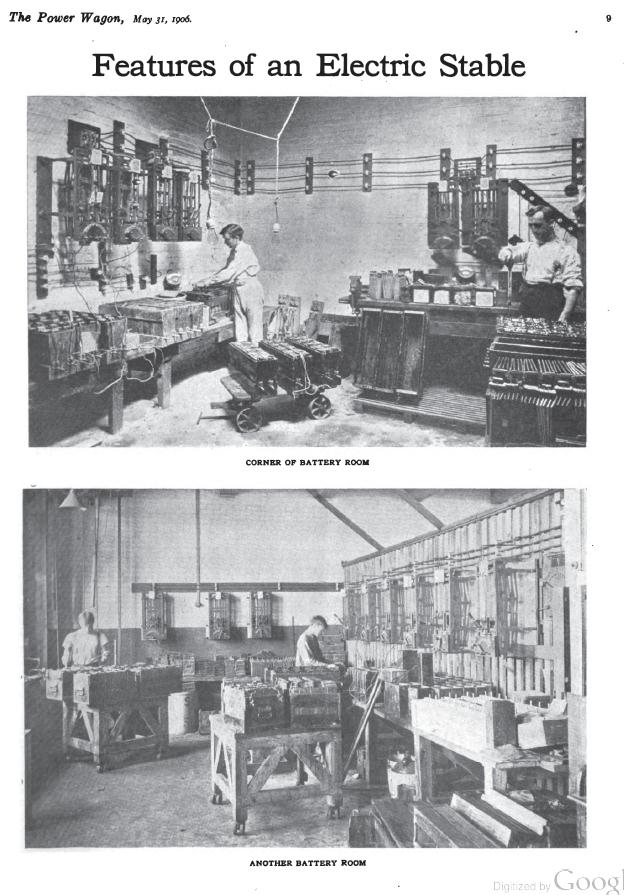
\includegraphics[width=\textwidth]{images/Laden_Batterieraum.jpg}
	\caption{Laden der Batterien in einem Batterieraum \cite{laden_alt}}
	\label{fig:Laden_Batterieraum}
\end{minipage}
\end{figure}
\end{landscape}

\subsection{Laden des Fahrzeuges zuhause}
Für das Laden zuhause gibt es ein zum \textsc{Detroit} passendes Ladegerät. Das beim Projekt untersuchte Modell "`Burtoni \& Rogers Junior Twin Six 12 Hour Charger"' besitzt die folgenden Daten:

\begin{tabular}{lll}
	\textbf{Originalbezeichnung} & \textbf{---\quad Deutsche Bezeichnung:} & \textbf{Wert} \\
	Volts A.C. & ---\quad Wechselspannung eingangsseitig: & $110$ V (US-amerikanisches Netz) \\
	Cycles & ---\quad Netzfrequenz: & $60$ Hz (US-amerikanisches Netz)\\
	Amps A.C. & ---\quad Wechselstrom eingangsseitig: & $12$ A \\
	Watts A.C. & ---\quad Leistung eingangsseitig: & $1050$ W \\
	Volts D.C. & ---\quad Gleichspannung ausgangsseitig: & $60$ V \\
	Amps D.C. & ---\quad Gleichstrom ausgangsseitig: & $12$ A \\
	Model & ---\quad Modelltyp: & JR-3 \\
	Ser. & ---\quad Seriennummer: & 19759
\end{tabular}

Wie man auf den ersten Blick erkennt, ist der Strom auf der Ein- und der Ausgangsseite der selbe. Das lässt darauf schliessen, dass sich dazwischen kein Transformator befindet. Durch einen ersten Gedanken zur Funktion resultierte also das in Abbildung \ref{fig:Ladegeraet1} gezeigte Schema:

\begin{figure}[h]
	\centering
		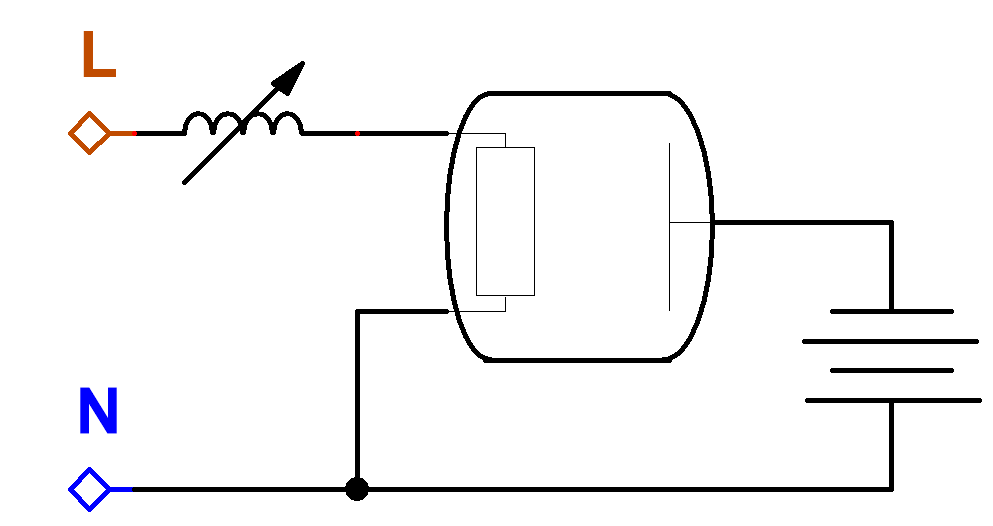
\includegraphics[width=0.60\textwidth]{images/Ladegeraet_Alt_1.PNG}
	\caption{Röhrengleichrichter mit einer Heizspannung von $230$ VAC}
	\label{fig:Ladegeraet1}
\end{figure}

Dabei wird zuerst der Stromfluss durch eine veränderbare Induktivität begrenzt. Eine anschliessende Gleichrichterröhre, deren Funktion weiter unten erklärt wird, sorgt dafür, dass nur die Halbwelle der gewünschten Polarität durchgeleitet wird. Dieser begrenzte Gleichstrom kann nun zum Laden der Batterie verwendet werden.

Die verwendete Gleichrichterröhre funktioniert dabei anders als die bereits vorgestellten Quecksilberdampfgleichrichter im Kapitel \ref{Laden_in_Garage}. In Gleichrichterröhren befindet sich ein Glühdraht, welcher gleichzeitig auch als Kathode fungiert. Dieser Glühdraht wird mittels einer Spannung beheizt, zusätzlich liegt an einem Ende das Kathodenpotential an. Durch die hohe Temperatur wird auch hier das Lösen von Elektronen ermöglicht, welche bei richtiger Spannungspolarität der Anoden-Kathodenspannung zur Anode beschleunigt werden. Da lediglich eine Halbwelle durchgeleitet wird, ist auch hier eine Gleichrichtung erfolgt. Eine der beiden im Ladegerät verbauten Gleichrichterröhren ist in Abbildung \ref{fig:Roehre_Diode} gezeigt: \newpage

\begin{figure}[h]
	\centering
		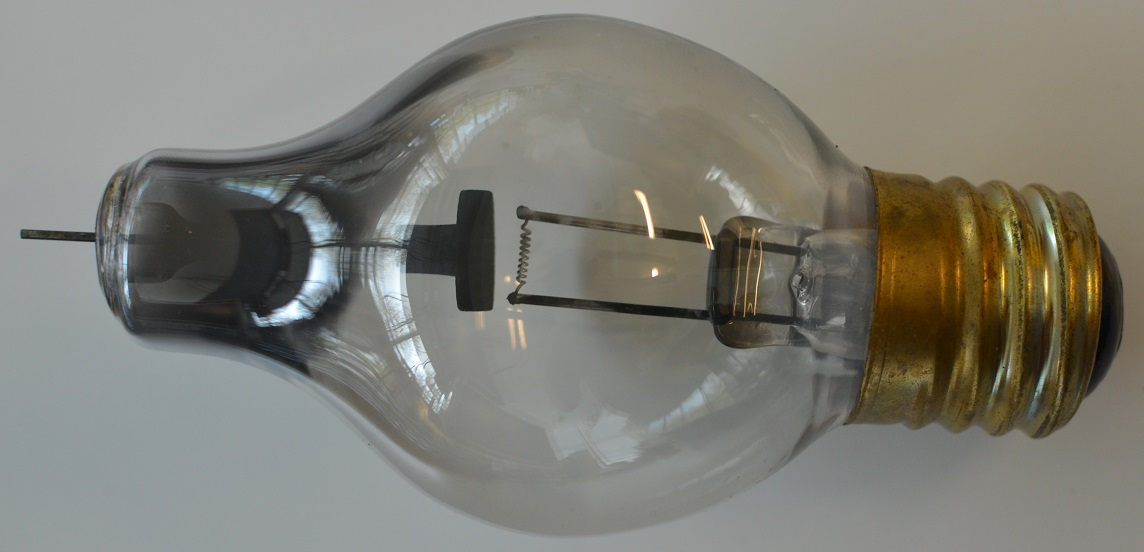
\includegraphics[width=0.75\textwidth]{images/Roehre_Diode.jpg}
	\caption{Gleichrichterröhre, auch Diode genannt}
	\label{fig:Roehre_Diode}
\end{figure}

Es konnte jedoch schnell gezeigt werden, dass dies nicht der im Ladegerät verbauten Schaltung entspricht. So ist zum einen auf dem Gehäuse die Bezeichnung "`Balanced Full Wave"' angebracht, was darauf hindeutet, dass beide Halbwellen gleichgerichtet werden. Zum anderen ist eine Anzeige vorhanden, mit der überwacht wird, dass beide Röhren gleich belastet werden. Dies ist ein Hinweis darauf, dass beide Röhren nicht nur parallel geschaltet sind, sondern sie je eine Halbwelle gleichrichten und bei ungleichmässigen Strömen das Eisen des Transformators asymmetrisch belastet wird. Aus diesen Überlegungen konnte die Schaltung des Netzgerätes hergeleitet werden. Das ist in Abbildung \ref{fig:Schema_Ladegeraet_Alt} gezeigt. Es handelt sich dabei um eine sogenannte Mittelpunktschaltung:

\begin{figure}[h]
	\centering
		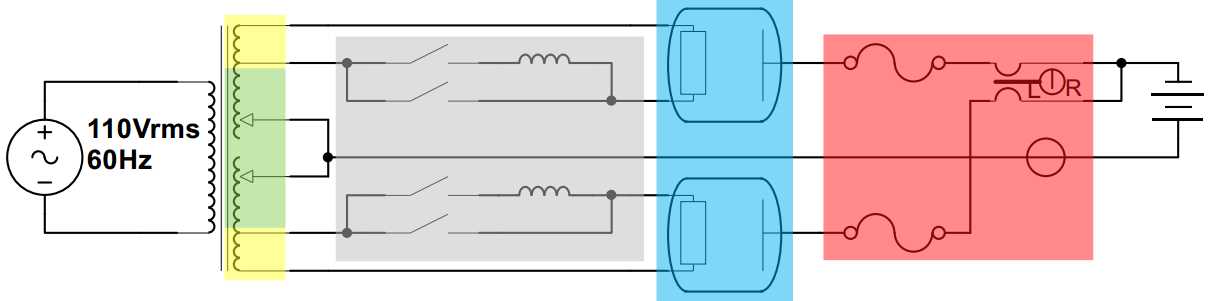
\includegraphics[width=1.00\textwidth]{images/Ladegeraet_Alt_2.PNG}
	\caption{Schaltung des originalen Netzgerätes}
	\label{fig:Schema_Ladegeraet_Alt}
\end{figure}

Es soll an dieser Stelle noch kurz die Funktion des Ladegerätes vorgestellt werden. Begonnen wird dabei mit der eingangsseitigen Transformatorenwicklung. Diese sorgt dafür, dass sämtliche Wicklungen auf der Sekundärseite ebenfalls Spannung abgeben können. Die ersten beiden dieser Wicklungen sind die gelb hinterlegten Heizwicklungen, gezeigt in Abbildung \ref{fig:Schema_Ladegeraet_Alt}. Diese sorgen dafür, dass die Heizwicklungen, die möglichst niederohmig sein sollen (um den gleichzurichtenden Stromfluss nicht zu bremsen), mit einer niedrigen Spannung versorgt werden können. Über die beiden grün gefärbten Transformatorenwicklungen lässt sich die Höhe der ausgangsseitigen Gleichspannung und damit am Ende auch der Gleichstrom regulieren. Dies geschieht über den Drehknopf, welcher sich mittig an der Front des Ladegerätes befindet.

\newpage

Der graue Bereich wird vom Schalter beeinflusst, welcher sich rechts an der Front befindet. So sind in der Aus-Stellung beide Schalter geöffnet, sodass keine Verbindung zur Batterie besteht. Bei Stufe eins von zwei wird der Stromfluss durch die Induktivität zusätzlich behindert, was in kleineren Strömen im Vergleich zu Stufe zwei resultiert, bei welcher die Induktivität überbrückt wird. Die Funktion der beiden Gleichrichterröhren wurde bereits erläutert. Sie sorgen dafür, dass jeweils nur eine Halbwelle durchgeleitet wird (die positive Halbwelle bei der unteren Röhre und die negative Halbwelle bei der oberen Röhre). Durch die Kombination der beiden Halbwellen erhält man eine pulsierende Gleichspannung, welche beide Halbwellen gleichrichtet.

Es folgen noch die rot hinterlegten Sicherheits- und Überwachungsbauteile. Die beiden Sicherungen sorgen dafür, dass kein zu grosser Strom zu den Batterien fliessen kann. Das Amperemeter zeigt den aktuellen Stromfluss an, sodass eventuell mit dem Transformator nachgeregelt werden kann. Interessant sind die beiden gekoppelten Spulen. Dazu werden die Anodenleitungen beider Röhren durch einen gemeinsamen Eisenkern geführt. Sind die Stromflüsse in beiden Röhren gleich, so wird keine Spannung induziert beziehungsweise ist deren Frequenz zu hoch, um das mechanische Anzeigegerät auszulenken. Ist der Stromfluss hingegen asymmetrisch, so wird eine Spannung induziert und dies auf dem Messgerät angezeigt. Dadurch wird darauf hingewiesen, dass der Transformator einseitig belastet wird.

Abschliessend soll noch ein Blick in das originale Ladegerät geworfen werden (siehe Abbildung \ref{fig:Ladegeraet_Original}):

\begin{figure}[h]
	\centering
		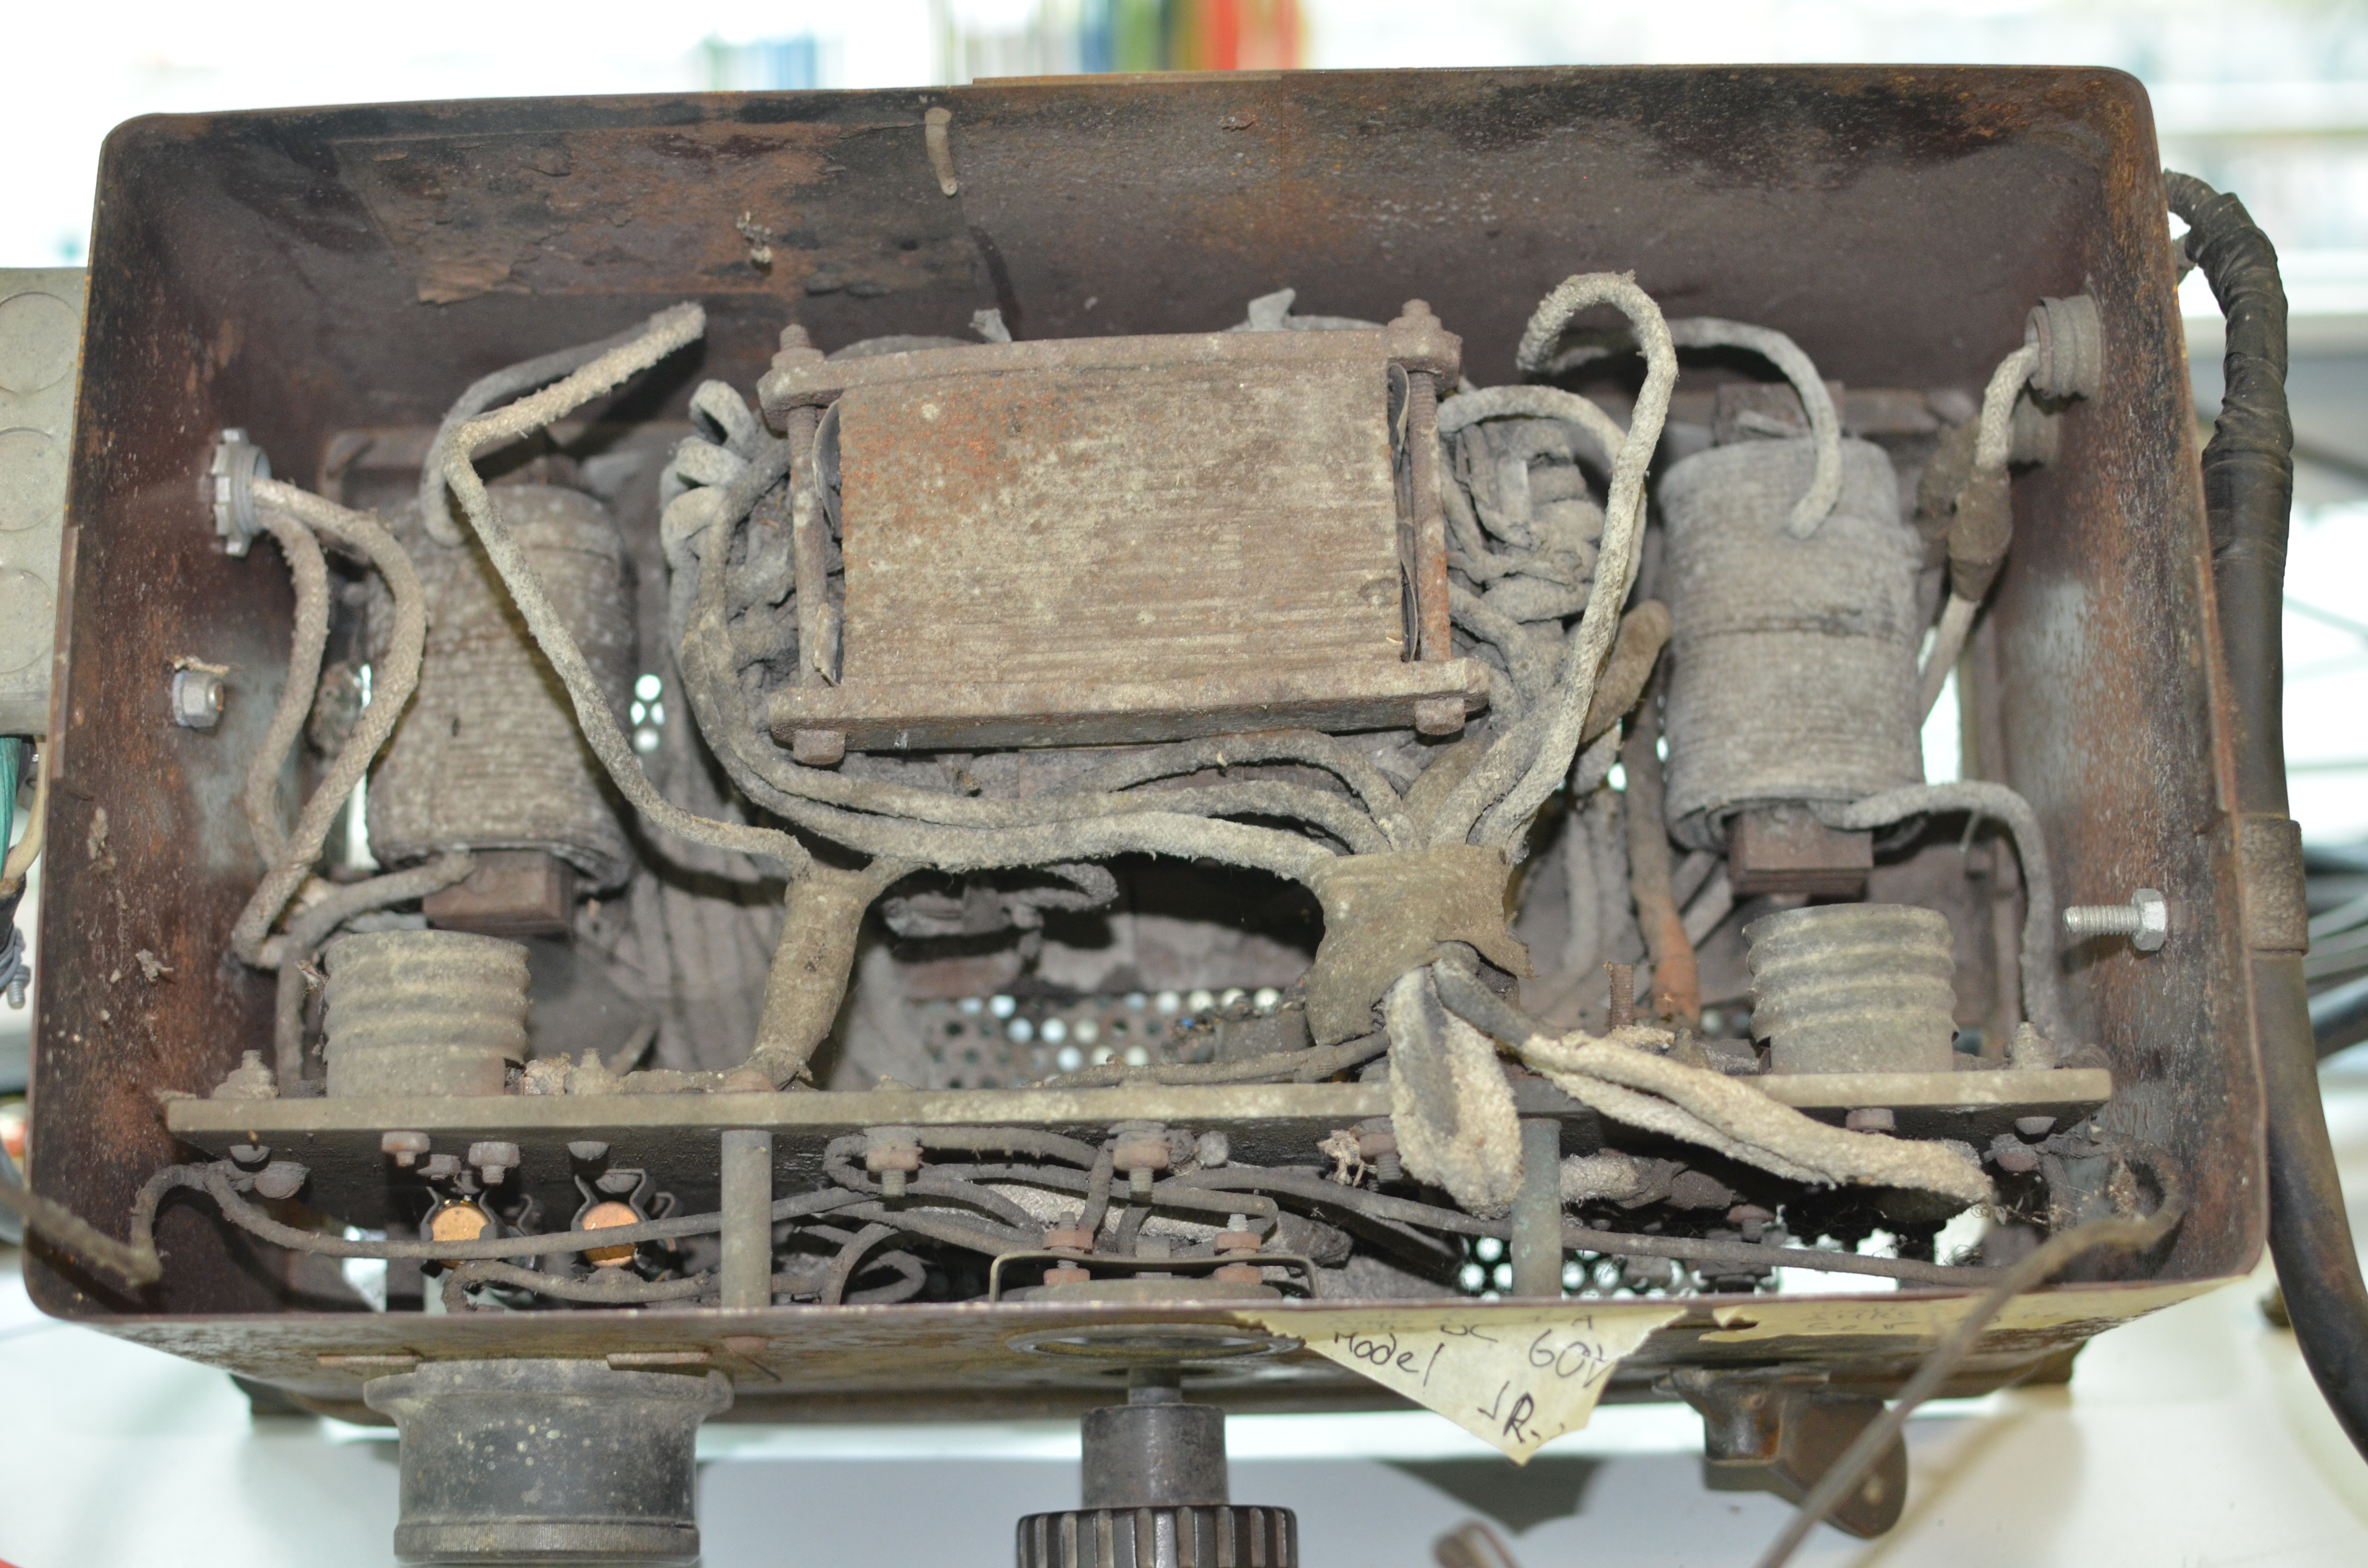
\includegraphics[width=0.95\textwidth]{images/Ladegeraet_Original.JPG}
	\caption{Das geöffnete originale Ladegerät von Oben betrachtet (1: Transformator, 2: Drosselspule, 3: Sockel für Gleichrichterröhren, 4: Umschalter Ladestufe, 5: Spannungsregelung Transformator, 6: Symmetrieüberwachung, 7:Ampèremeter)}
	\label{fig:Ladegeraet_Original}
\end{figure}

\newpage
\section{Alternative Konzepte zur Spannungsregelung}
Da zu Beginn des Projektes noch nicht klar war, um welches Modell es sich beim Detroit genau handelt, wurde zu Beginn eine alternative Schaltung untersucht. Beim Besuch des Museums von Hanspeter Setz konnte ein Rauch und Lang begutachtet werden, bei dem wieder eine andere Schaltung verwendet wurde. Auf diese beiden Schaltungen mit ihren Vor- und Nachteilen soll an dieser Stelle kurz eingegangen werden.

\subsection{Detroit Modell 68}
Als zu Beginn des Projektes das Fahrzeug noch nicht besichtigt werden konnte, wurde mit den bereits vorhandenen Informationen nach der Schaltung gesucht. Dabei wurde vor allem eine Schaltung untersucht, die sich jedoch am Ende als die Falsche heraus gestellt hat. Diese Schaltung soll aber trotzdem hier vorgestellt werden, da sie eine alternative Möglichkeit des selben Herstellers darstellt.

Der Detroit Modell 68 besass eine Batterie mit zwei Zwischenabgriffen, sodass insgesamt drei Spannungen zur Verfügung standen. Diese Spannungen wurden für verschiedene Fahrstufen zur Verfügung gestellt. Die Spannung stieg über die Zwischenabgriffe linear an, bis bei der obersten Stufe $84$ V erreicht wurden. Es ist jedoch nicht bekannt, ob die Batterien unterschiedliche Kapazitäten besassen, um die ungleiche Entladung auszugleichen.

Das Funktionsprinzip dieser Schaltung ist bestechend einfach. Steigt doch mit zunehmender Spannung auch die induzierte Spannung, welche für die Geschwindigkeit verantwortlich ist. Auch sind höhere Leistungen bei höheren Stufen möglich (der Strom wird als limitiert angenommen), womit beispielsweise der grössere Luftwiderstand oder das schnellere Bergauffahren ausgeglichen wird. Nachteilig an dieser Schaltung ist auf jeden Fall die Batterie, die je nach Fahrstufe anders und dadurch ungleichmässig entladen wird. Dadurch ist meist nicht die volle Kapazität der Batterien nutzbar. Einzige Ausnahme wäre der Fall, dass die niedrigeren Stufen lediglich zum Anfahren benötigt werden, anschliessend jedoch mit der höchsten Stufe gefahren wird.

Für diese Batterie wurde bereits eine Schaltung angedacht, die es unter Zuhilfenahme von Dioden ermöglicht, sechs gleich grosse Batterien gleichmässig zu entladen. Die Batterien sind dabei entweder zu dritt in Serie (je zwei parallel), zu zweit in Serie (je drei parallel) oder komplett parallel verschaltet. Diese Schaltung ist in Abbildung \ref{fig:68} gezeigt.

\begin{figure}[h!]
	\centering
		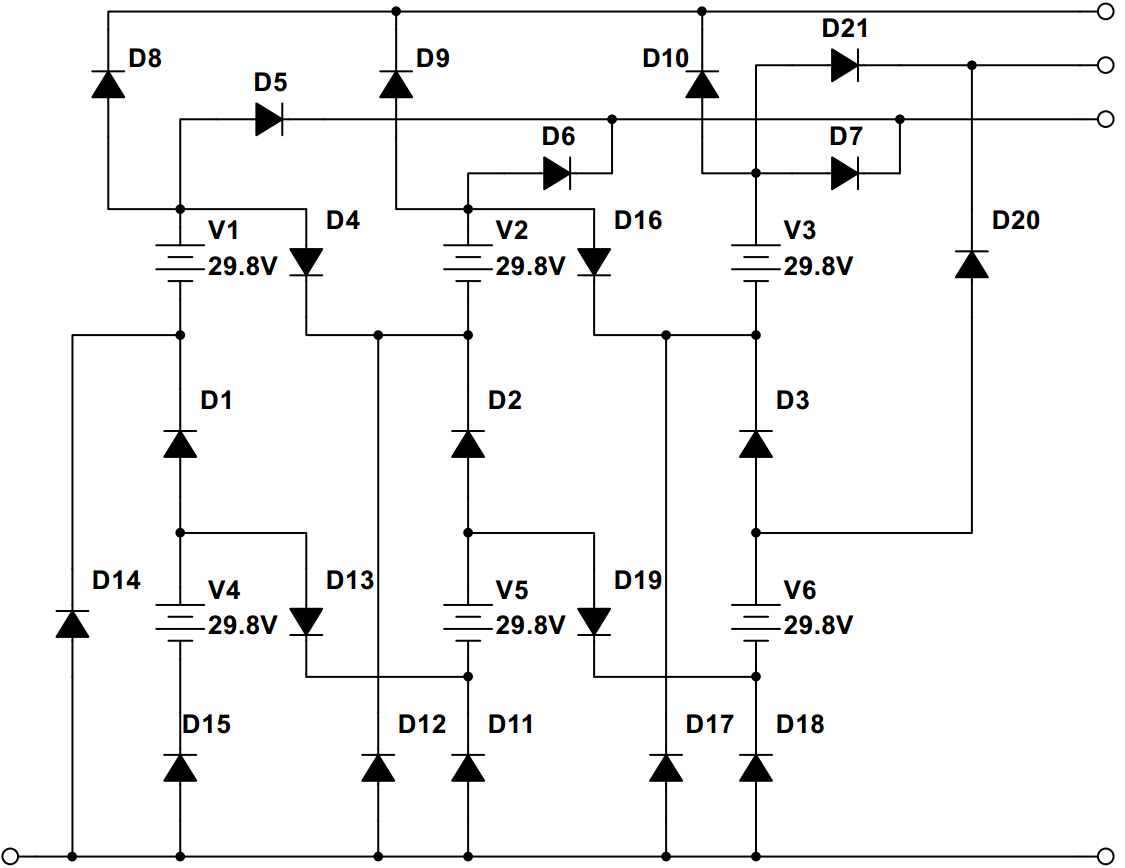
\includegraphics[width=0.75\textwidth]{images/68.PNG}
	\caption{Schaltung für eine Batterie mit Zwischenabgriffen}
	\label{fig:68}
\end{figure}

Mit dieser Schaltung sowie den Batterien des Peugeots wären Spannungen von $0\cdot29.8$ V$=0$ V, $1\cdot29.8$ V$=29.8$ V, $2\cdot29.8$ V$=59.6$ V und $3\cdot29.8$ V$=89.4$ V möglich gewesen, was sehr nahe an den originalen Spannungen gelegen hätte.

\subsection{Rauch und Lang}
Dieses Fahrzeug verfügt über eine sehr einfache Steuerung der Geschwindigkeit. Dazu werden seriell zum Motor verschieden grosse Widerstände hinzugeschaltet, die so die maximal induzierte Spannung im Motor verringern. Auch bei diesem Fahrzeug waren jedoch nur wenige einzelne Fahrstufen vorhanden, wobei der Hebel für jede Stufe ein anderes Plättchen im Schaltkasten herunter drückte, welches den entsprechenden Widerstand mit dem Anker verband. Das Fahrzeug ist in Abbildung \ref{fig:Setz} gezeigt.

\begin{figure}[p]
	\centering
		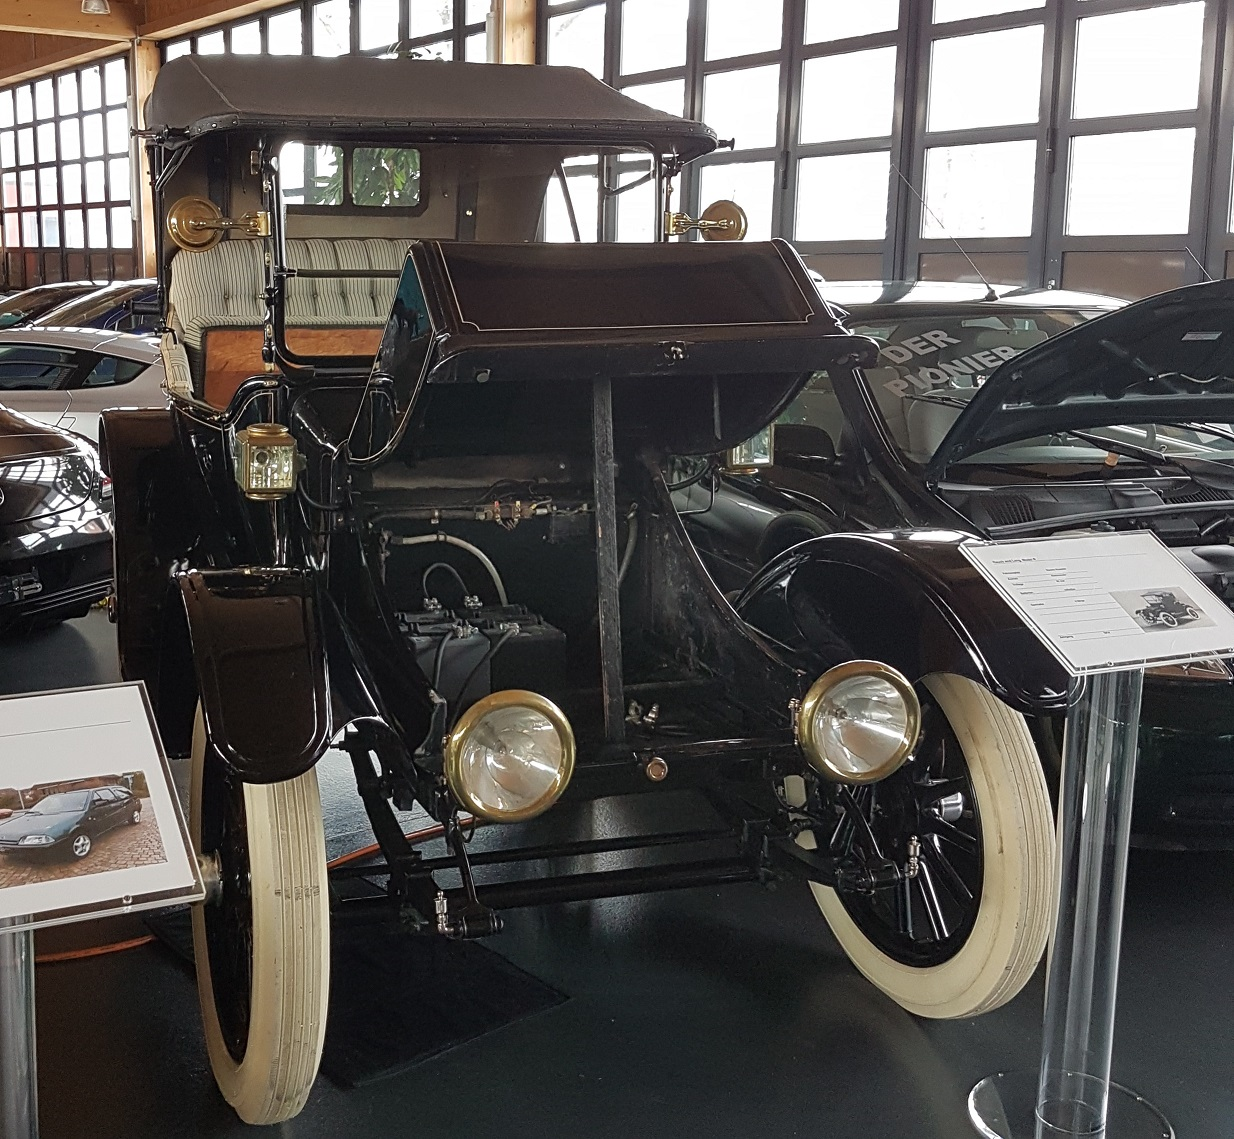
\includegraphics[width=0.9\textwidth]{images/Setz.JPG}
	\caption{Der Rauch und Lang im Museum von Herr Setz}
	\label{fig:Setz}
\end{figure}

Dadurch, dass in beinahe allen Stufen ein zusätzlicher Widerstand zum Motor geschaltet ist, entstehen zusätzliche Verluste im Auto, was die maximale Reichweite reduziert. Auch ist diese Schaltung nicht viel einfacher aufgebaut als die Schaltung des Detroits. Lediglich die Auftrennung auf zwei Batterien entfällt. Anstelle der zusätzlichen Motoranzapfungen für die Feldansteuerungen sind in dieser Schaltung weitere Widerstände nötig. Das Verständnis der Schaltung ist aber bedeutend einfacher: Ein grösserer Widerstand in Serie behindert den Stromfluss zum Motor stärker als ein kleiner Widerstand, sodass dadurch sehr einfach die Leistung reguliert werden kann. Im Gegensatz zur Schaltung des Detroits steigen aber hier das maximale Moment und die erreichbare Geschwindigkeit (bei gegebenem Gegenmoment) mit den höheren Stufen an, da der serielle Widerstand sowohl den maximalen Strom limitiert (beziehungsweise den Stromfluss entsprechend verhindert), als auch die maximal induzierte Spannung bei gegebenem Strom verringert.
\clearpage{\pagestyle{empty}\cleardoublepage}

\chapter{Das Peugeot-Unfallauto}
Um den Detroit batterietechnisch auf den aktuellsten Stand zu bringen, sollten aus einem Umfallauto die Batterie sowie die dazugehörigen Bauteile entnommen werden. Beim Unfallauto handelte es sich um einen Peugeot Ion. Dieses Kapitel soll zum einen aufzeigen, wie der Peugeot funktioniert, da dessen Funktionsweise sich stark von der des Detroits unterscheidet. Zum anderen soll ebenfalls aufgezeigt werden, welche Bauteile aus welchen Gründen für den Detroit übernommen oder nicht übernommen wurden.

\section{Batterie}
Beim Peugeot lag das Hauptaugenmerk auf der Batterie. Bei dieser handelte es sich um insgesamt 22 Viererblöcke vom Typ LEV50-4 \cite{lev50}. Jede Einzelzelle verfügt dabei über eine Kapazität von $50$ Ah bei einer Nennspannung von $3.7$ V. Da alle Zellen in Serie geschaltet waren, ergab sich eine Gesamtspannung von $22\cdot 4\cdot 3.7$ V$=325.6$ V. Zusammen mit der gleich gebliebenen Kapazität ergibt sich ein theoretischer Energiegehalt der Batterie von $325.6$ V$\cdot50$ Ah$=16.28$ kWh.

Auf jedem solchen Viererblock befand sich eine Sensorplatine des Batteriemanagementsystemes. Bereits auf dieser Platine wurden die Spannung sowie die Temperatur der einzelnen Zellen ausgewertet. Auch Balancierströme konnten auf diesen Platinen aktiviert werden. Eine solche Platine ist in Abbildung \ref{fig:BMS_Alt} zu sehen:

\begin{figure}[h!]
	\centering
		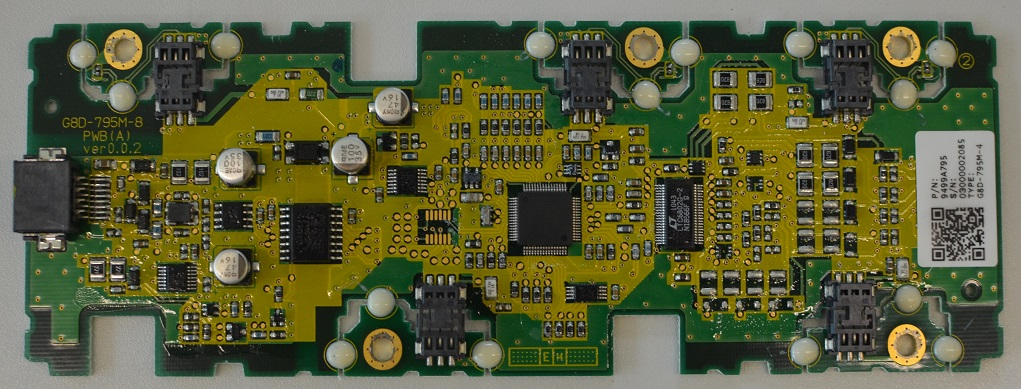
\includegraphics[width=0.80\textwidth]{images/BMS_Alt.JPG}
	\caption{Im Peugeot verbaute BMS-Sensorplatine}
	\label{fig:BMS_Alt}
\end{figure}

Die so gesammelten Daten wurden über eine proprietäre Verbindung an das Steuergerät übertragen, welches die Aufgabe hatte, die ausgewerteten Daten zu überwachen und gegebenenfalls Balancierströme oder weitere Schutzfunktionenen zu schalten.

Da es nicht möglich war, auf die so gesammelten Daten zuzugreifen, musste dieser Teil der Batterie ersetzt werden und es konnten nur die Zellen alleine übernommen werden.


\newpage
\section{Stromrichter und Motor}
Die Funktionsweise des Peugeots unterscheidet sich stark von der des \textsc{Detroits}. Aus diesem Grund soll an dieser Stelle ebenfalls kurz auf den Peugeot eingegangen werden, um aufzuzeigen, welche Lösung bei modernen Elektrofahrzeugen gewählt wird. Die Lösung des Peugeots kann stellvertretend für die meisten anderen modernen Elektrofahrzeuge präsentiert werden, da alle auf einem ähnlichem Prinzip beruhen. Selbst moderne Eisenbahnfahrzeuge sind ähnlich aufgebaut, jedoch mit einem grossen Unterschied: Die Energie wird nicht als Gleichspannung aus einer Batterie geliefert, sondern kommt (als Gleich- oder Wechselspannung) meist mit höherer Spannung aus einem Fahrdraht.

Im Gegensatz zum \textsc{Detroit}, der eine klassische Gleichstrommaschine verwendet, ist der Peugeot mit einer Drehfeldmaschine ausgerüstet. Diese Motoren besitzen gegenüber der Gleichstrommaschine mehrere Vorteile. Durch den Wegfall der Bürsten (Asynchronmaschine und permanenterregte Synchronmaschine) beziehungsweise durch deren deutlich geringerer Belastung (Synchronmaschine) kann die Wartung reduziert werden. Auch sind, insbesondere bei Synchronmaschinen, bei gleicher Leistung kompaktere Motoren im Vergleich zur Gleichstrommaschine möglich.

Im klassischen Fall werden Synchronmaschinen nicht als Motor, sondern in Kraftwerken als Generator verwendet. Der Asynchronmotor hingegen ist die Standardmaschine am dreiphasigen Netz (Drehstrom), wie es in der Schweiz vorhanden ist. Durch das Aufkommen von Stromrichtern, die es einfach ermöglichen Wechselspannung in Gleichspannung und umgekehrt umzuwandeln und folglich auch Wechselspannung einer Frequenz in Wechselspannung einer anderen Frequenz (über den Zwischenschritt der Gleichspannung) wurde beiden Maschinentypen ein weiteres Anwendungsgebiet eröffnet. Dies ist bei drehzahlvariablen Antrieben.

Ein solcher Stromrichter ist auch im Peugeot eingebaut. Da aus der Batterie bereits Gleichspannung bezogen wird, entfällt im Vergleich zum Frequenzumrichter die erste Stufe der Gleichrichtung. Ein Beispiel für einen Stromrichter, wie er im Peugeot verwendet wird, ist in Abbildung \ref{fig:Bruecke} gegeben.

\begin{figure}[h!]
	\centering
		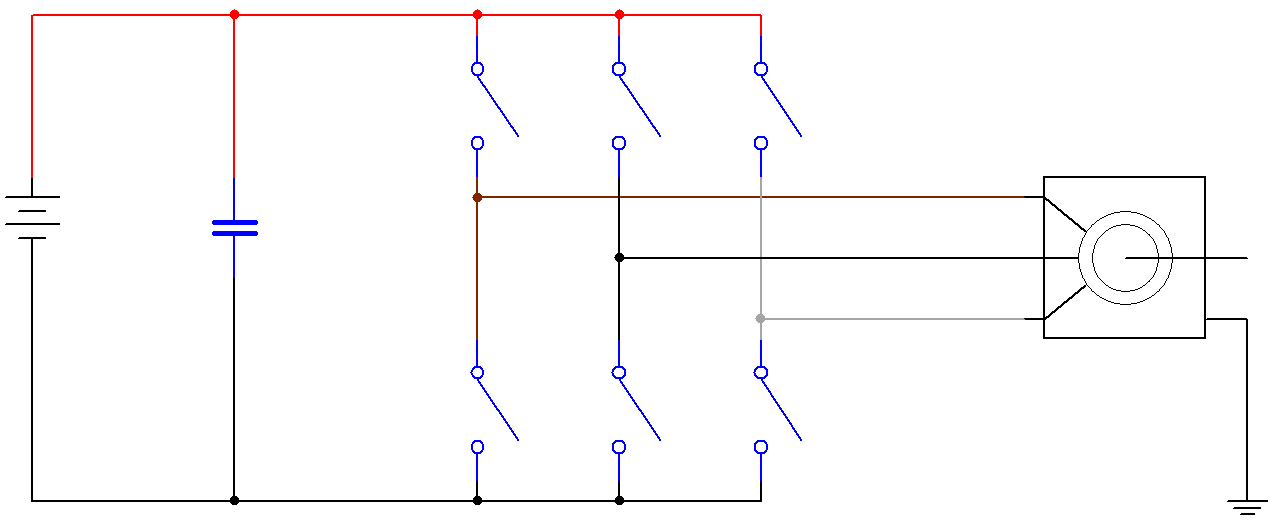
\includegraphics[width=0.80\textwidth]{images/Bruecke.PNG}
	\caption{Aufbau einer dreiphasigen Brücke}
	\label{fig:Bruecke}
\end{figure}

\newpage

Die sechs Transistoren dienen dabei als Schalter, können also nur ein- oder ausgeschaltet sein. In jedem senkrechten Pfad ist nur jeweils ein Schalter eingeschaltet, da es ansonsten zu einem Kurzschluss kommen würde. Durch die beiden Schalter kann der jeweilige Abgang entweder auf den positiven oder den negativen Anschluss der Batterie gelegt werden. Wird dies genügend schnell durchgeführt und der Abgang anschliessend gemittelt (dies kann durch die Induktivität des Motors angenommen werden), so kann dabei jede beliebige Spannungsform erreicht werden. Ein einfaches Beispiel für das Resultat dieser Schaltung kann die Nachbildung des Drehstromnetzes, wie wir es vom schweizerischen Landesnetz kennen, sein. Mit diesem sogenannten Drehfeld kann der Motor in Bewegung gesetzt werden. In Abbildung \ref{fig:Phasenspannungen} ist ein sogenannter Dreiphasendrehstrom dargestellt. Die Spannungen der einzelnen Phasen sind dabei um $120^\circ$ phasenverschobene Sinusfunktionen.

\begin{figure}[h!]
	\centering
		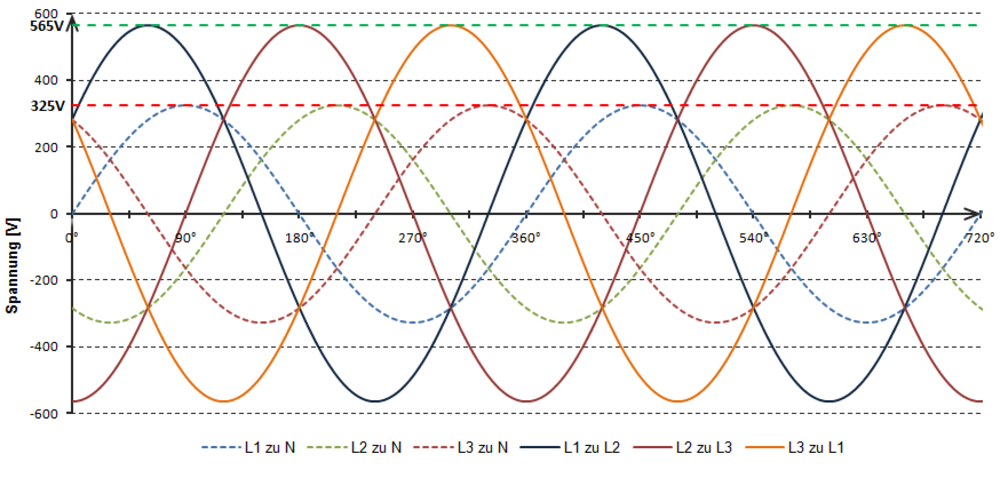
\includegraphics[width=1.00\textwidth]{images/Phasenspannungen.PNG}
	\caption{Phasenspannungen und verkettete Spannungen am Beispiel des $400$ VAC/$50$ Hz-Drehstromnetzes \cite{phasen}}
	\label{fig:Phasenspannungen}
\end{figure}

Drehfeldmaschinen bieten gegenüber Gleichstrommaschinen einen weiteren Vorteil: Wird eine Ausgangsfrequenz des Stromrichters eingestellt, so dreht sich die Maschine ebenfalls mit dieser Frequenz (Synchronmaschine) beziehungsweise aufgrund des Schlupfes um einige Prozent langsamer (Asynchronmaschine). Versucht nun der Motor, durch aufgenommene Leistung an der Welle, schneller zu drehen als das Feld, so wird er automatisch zum Generator und bremst dabei das Fahrzeug. Dabei muss dieser Vorgang für beide Motorentypen unterschieden werden.

Bei \textbf{Asynchronmaschinen} dreht sich funktionsbedingt der Rotor immer etwas langsamer als das Feld, diese Differenz wird auch Schlupf genannt. Ist die Maschine im Nennbetrieb, so kann die Vereinfachung getroffen werden, dass das abgegebene Moment proportional zum Schlupf ist. Folglich ist also bei gleicher Drehzahl kein Moment mehr an der Welle abgreifbar. Wird die mechanische Drehzahl grösser als die sogenannte Synchronfrequenz (bei der Synchronfrequenz tirtt kein Schlupf auf, Netz- und Drehfrequenz sind also identisch), so wird der Schlupf negativ und folglich auch das Moment an der Welle. Die Maschine nimmt also mechanische Leistung auf und gibt diese als elektrische Leistung ab.

\textbf{Synchronmaschinen} funktionieren anders als Asynchronmaschinen. Der Name kommt daher, dass sie stets mit der selben Drehzahl wie das Feld drehen. Ähnlich wie beim Schlupf der Asynchronmaschine gibt es auch hier eine das Moment beeinflussende Grösse. Im Motorbetrieb läuft der Rotor dem Statorfeld hinterher. Der Winkelversatz ist dabei verantwortlich für das abgegebene Moment (beziehungsweise umgekehrt, das Moment bestimmt den Winkelversatz). Wird dieser Winkelversatz null, der Stator läuft also exakt mit dem Rotorfeld mit, so ist auch das abgegebene Moment null. Wenn der Rotor dem Drehfeld voraus eilt, so ändert sich auch hier die Richtung des elektrischen Energieflusses.

Die so erzeugte Energie ist in beiden Fällen eine dreiphasige Wechselspannung. Mit Hilfe des Stromrichters wird dadurch wieder eine konstante Gleichspannung erzeugt, mit welcher beim Bremsen die Batterie aufgeladen werden kann (dies wird auch als Rekuperation bezeichnet). Dadurch kann zur Bremsung des Fahrzeuges einfach die Frequenz unterhalb der Motorendrehzahl gehalten werden (Asynchronmaschine) beziehungsweise, bildlich gesprochen, "`kurz gewartet werden"', bis der Rotor dem Drehfeld voreilt (Synchronmaschine).

Die hier vorgestellten Vorgänge benötigen ein hohes Mass an Regelung. Zusätzlich zu den Schaltelementen kommt in jedem Stromrichter noch ein Prozessor hinzu, der den gesamten Zustand regelt. Auch sind viele weitere Schaltungsteile nötig, um beispielsweise eine galvanische Trennung, eine Messung der elektrischen Grössen oder die Überwachung der Schaltertemperaturen durchzuführen. Diese sollen jedoch an dieser Stelle nicht weiter behandelt werden. Es sollte nur die grundsätzliche Funktionsweise des Stromrichters erklärt werden.

Auch Gleichstrommaschinen, wie die im \textsc{Detroit} verbaute, können als Generator benutzt werden. Beim \textsc{Detroit} war dies jedoch trotzdem nicht möglich. Für genauere Informationen sei auf das Kapitel \ref{bremse} verwiesen.
%Natürlich kann auch eine Gleichstrommaschine als Generator benutzt werden. Zu diesem Zweck muss die induzierte Spannung (siehe Kapitel \ref{gm}) grösser werden als die Batteriespannung. Da sich dadurch aber auch die Stromrichtung umdreht, wird bei der Reihenschlussmaschine das Erregerfeld ebenfalls gekehrt, was die Nutzung als Generator verhindert. Für die Nutzung als Generator wäre also eine fremderregte Maschine benötigt worden. Dies wäre beim \textsc{Detroit} schaltungstechnisch möglich gewesen, aufgrund der stark variierenden Drehzahlen wäre jedoch ebenfalls ein Stromrichter nötig gewesen, um die Spannung des Generators an die Batteriespannung anzupassen.

Für weitere, ausführlichere Informationen zu Drehfeldmaschinen und die dazugehörigen Stromrichter sei auf die Literatur \cite{elektrischeantriebe} verwiesen.

\newpage
\section{Lademodi}
Der Peugeot konnte auf zwei verschiedene Arten geladen werden. Zum einen besitzt er ein internes Ladegerät. Mit einem Hilfskabel kann die Verbindung zum $230$ VAC-Netz hergestellt werden, dessen Spannung im Peugeot selbst auf die benötigte Gleichspannung umgesetzt wird. Alternativ kann unter Umgehung des internen Gleichrichters direkt mit Gleichstrom geladen werden, was höhere Ladeleistungen ermöglicht.

\paragraph{Laden am 230 VAC-Netz}
Zum Anschluss am Wechselspannungsnetz ist ein Hilfskabel nötig. Dieses Hilfskabel bildet zum einen den Übergang zwischen den verschiedenen Steckersystemen. Zum anderen ist in ihm auch eine elektrische Schaltung eingebaut. Diese findet ihren Platz in einer Box in der Mitte des Kabels. Diese Schaltung übernimmt dabei sowohl Schutzaufgaben (Überspannungs- und Überstromschutz), als auch die Kommunikation mit dem Fahrzeug. So teilt die Schaltung dem Fahrzeug den maximal beziehbaren Strom mit (dieser ist ja unter Umständen durch die verwendete Steckdose bestimmt). Ausserdem sind in dieser Box mehrere Leuchtdioden verbaut, die den Zustand des Fahrzeuges sowie eventuelle Fehler anzeigen. Das vorliegende Hilfskabel ist für eine haushaltsübliche Steckdose mit $230$ VAC und $10$ A gedacht. Es gibt jedoch insbesondere bei öffentlichen Ladestationen auch stärkere Anschlüsse, welche Dreiphasenwechselstrom übertragen. Dieses Hilfskabel mit Box ist in Abbildung \ref{fig:Hilfskabel} zu sehen:

\begin{figure}[h]
	\centering
		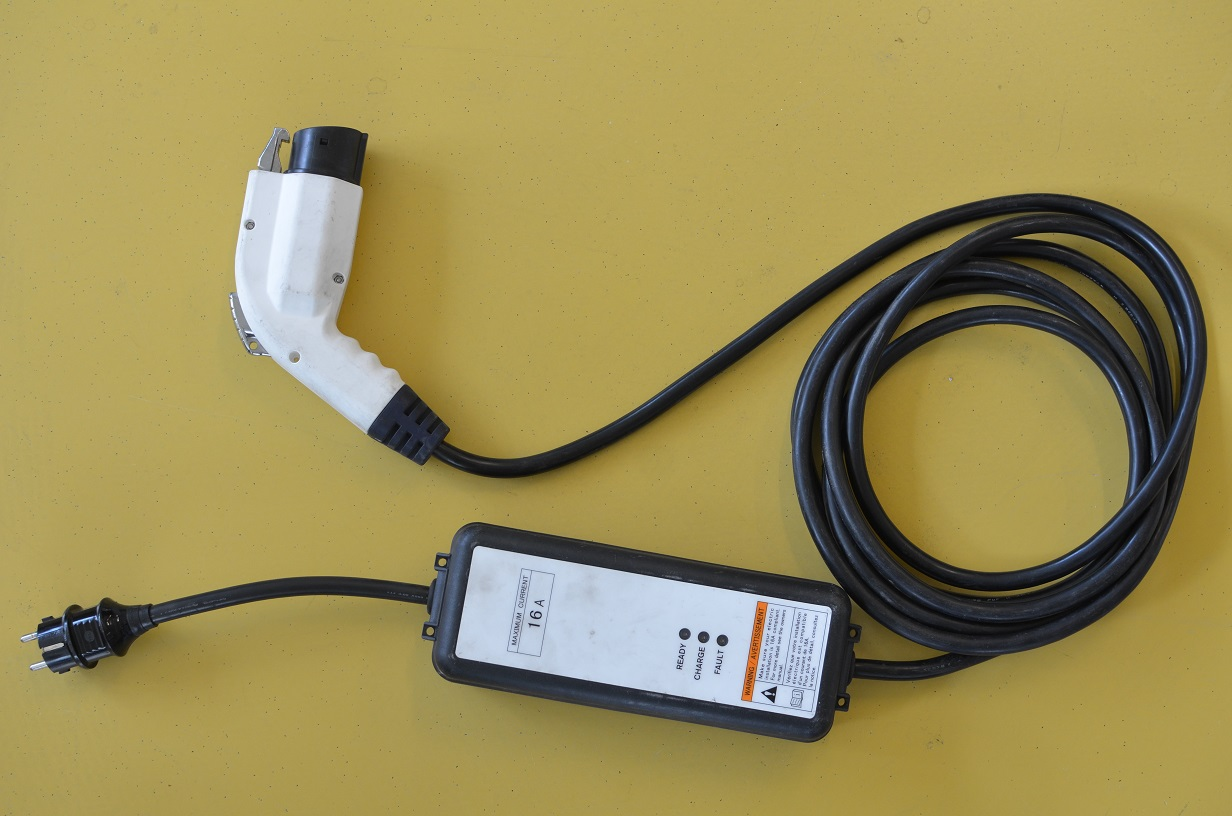
\includegraphics[width=0.80\textwidth]{images/Hilfskabel.JPG}
	\caption{Das verwendete Hilfskabel zum Laden mit $230$ VAC}
	\label{fig:Hilfskabel}
\end{figure}

\newpage

Bei dieser Ladeart ist das gesamte Ladegerät innerhalb des Peugeots untergebracht. Auf dieses Ladegerät soll folgend eingegangen werden, zuerst sollen jedoch die Funktionen des Ladegerätes mithilfe von Abbildung \ref{fig:Laden_Peugeot} erläutert werden:

\begin{figure}[h]
	\centering
		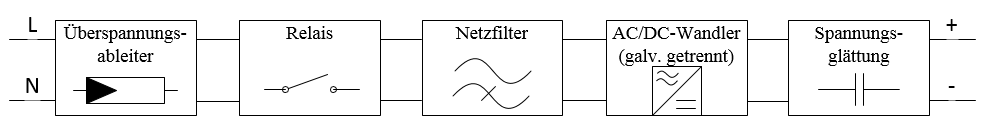
\includegraphics[width=1.00\textwidth]{images/Laden_Peugeot.PNG}
	\caption{Ablauf beim Laden des Peugeots am $230$ VAC Netz}
	\label{fig:Laden_Peugeot}
\end{figure}

Am Beginn steht die Schutzschaltung im Hilfskabel, welches bereits vorgestellt wurde. Das erste im Fahrzeug befindliche Bauteil ist ein Hauptrelais, welches die Ladung des Fahrzeuges ein- und ausschalten kann. Dieses Relais kann auch über das Hilfskabel geschaltet werden, sodass bei einem externen Fehler die Ladung abgebrochen werden kann. Als erste Stufe der eigentlichen Schaltung kann das Netzfilter gesehen werden. Mit Hilfe von Spulen und Kondensatoren sorgt dieses dafür, dass möglichst wenig Blindleistung aus dem Netz bezogen wird. Diese Blindleistung wird nämlich von dem Diodengleichrichter erzeugt, der dem Filter folgt. Diese Spannung wird durch den Gleichspannungswandler, welcher nachfolgend noch detaillierter vorgestellt wird, auf den zur Batterie passenden Wert gebracht. Am Ende erfolgt noch eine Glättung der Ausgangsspannung, dies erfolgt mittels eines Kondensators.

Die Ausgangsspannung der Diodenbrücke weist mehrere Nachteile auf. Die grössten Nachteile sind die fehlende galvanische Trennung, die proportionale Abhängigkeit zur Netzspannung, sowie die fehlende Möglichkeit zur Regelung. Ausserdem entspricht der Wert dieser Spannung nicht dem Wert, welcher die Batterie benötigt. Aus all diesen Gründen ist zwischen dem Diodengleichrichter und der Batterie ein Gleichspannungswandler eingebaut, der die zuvor beschriebenen Nachteile eliminiert. Die Schaltung des Starkstrompfades ist in Abbildung \ref{fig:Ladegeraet_Peugeot} abgebildet:

\begin{figure}[h]
	\centering
		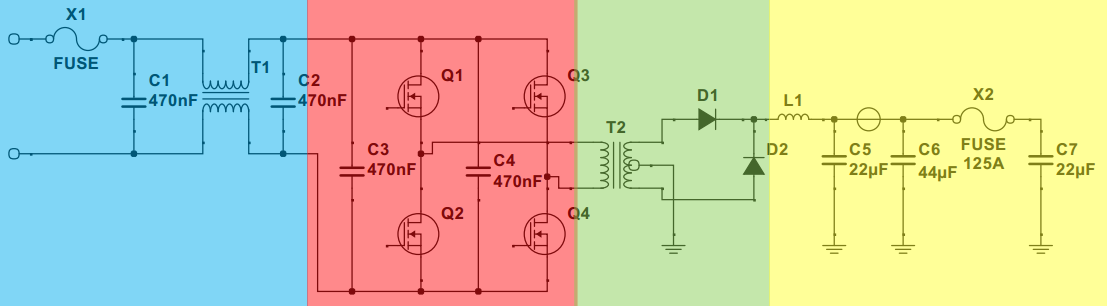
\includegraphics[width=1.00\textwidth]{images/Ladegeraet_Peugeot.PNG}
	\caption{Gleichspannungswandler im Ladegerät des Peugeots}
	\label{fig:Ladegeraet_Peugeot}
\end{figure}

Auch bei dieser Schaltung erfolgt eine eingangsseitige Glättung durch ein Filter, in der Abbildung blau dargestellt. Da die Eingangsspannung jedoch direkt von der Diodenbrücke, die bereits über eine kapazitive Glättung verfügt, erfolgt, konnte der Sinn dieses Filters nicht geklärt werden. Eine Idee wäre jedoch, dass unter Umgehung des Diodengleichrichters direkt mit einer Gleichspannung gespeist werden kann, \textcolor{blue}{oder aber dass das eingekaufte Bauteil einfach so ausgelegt ist}. Die beiden Kondensatoren sorgen für gleichmässige Spannungen am Ein- und Ausgang. Die gekoppelten Spulen sorgen dafür, dass sich bei schnell ändernden Strömen eine Gegenspannung einstellt.

Im roten Bereich befinden sich die vier Leistungs-MOSFETs vom Typ 2SK3697 \cite{2sk3697}. Diese vier Halbleiter erzeugen aus der Gleichspannung wieder eine Wechselspannung, allerdings mit deutlich höherer Frequenz als die Netzfrequenz. Dadurch kann der nachfolgende Transformator verkleinert ausgeführt werden. Parallel zu jeder Halbbrücke ist jeweils ein Kondensator eingebaut, der Spannungsabfälle bei den Schaltvorgängen abdämpft. Diese Wechselspannung kann durch Polaritätswechsel der Gleichspannung erzeugt werden, indem zwischen den Schaltzuständen "`$Q_1$ und $Q_4$ eingeschaltet"' und "`$Q_2$ und $Q_3$ eingeschaltet"' gewechselt wird. Sind die beiden oberen oder unteren Transistoren eingeschaltet, so ist die Ausgangsspannung der Brücke $0$ V. Durch abwechselnde Benutzung der Schaltzustände kann also sowohl die Frequenz als auch die Spannung der Brücke verändert werden. Begrenzt wird dies lediglich durch die maximale Schaltfrequenz der Transistoren und der eingangsseitigen Gleichspannung.

Um eine galvanische Trennung und eventuell auch eine Spannungsanpassung zu ermöglichen, ist die grün hinterlegte Transformatorenschaltung eingebaut. Die Mittelanzapfung mit den beiden Dioden sorgt dafür, dass beide Halbwellen wieder gleichgerichtet werden können (im Vergleich zu einer Diodenbrücke können aber zwei Dioden eingespart werden). Dadurch kann der Eisenkern gut entmagnetisiert werden. Die induzierte Spannung entsteht je nach Polarität in der oberen oder der unteren Halbwicklung.

Auch ausgangsseitig wird die erhaltene Spannung geglättet, da sie ja vom Transformator her eine Welligkeit aufweist. Dies ist im gelben Bereich gezeigt und geschieht durch eine Spule und mehrere Kondensatoren. Nach dem ersten Tiefpass folgt ausserdem eine Strommessung, mit welcher schlussendlich die Regelung der MOSFETs beeinflusst wird. Ausserdem ist ausgangsseitig noch eine handelsübliche Kfz-Streifensicherung verbaut. Wird der Nennstrom dieser Sicherung ($125$ A) und auch die Abmessungen der übrigen Schaltungsteile berücksichtigt, so sieht man sehr gut, dass diese Schaltung für höhere Ströme als die $10$ A des Hilfskabel ausgelegt ist. Auch die aktive Wasserkühlung der gesamten Schaltung deutet dies an. So gibt Peugeot für das Modelljahr 2011 an, dass die $16.28$ kWh Batterie innerhalb von 20 Minuten zur Hälfte geladen werden kann \cite{ion}. Dies entspricht einer Ladeleistung von $24.42$ kW, wobei bei einem idealen Gleichrichter auf der Wechselspannungsseite ein Strom von $35.39$ A resultieren würde (dreiphasig). Werden zusätzlich Verluste und Blindleistung berücksichtigt, so erscheint ein Ladestrom von $40$ A, was einer Normsicherungsgrösse entsprechen würde, als realistisch.

\paragraph{Ladung mit Gleichstrom}
Das interne Netzgerät des Peugeots kann auch umgangen werden. Zu diesem Zweck besitzt der Peugeot einen sogenannten ChaDeMo-Anschluss, mit welchem direkt mittels Gleichstrom die Batterie geladen werden kann \cite{chademo}. Dieser Anschluss überträgt ausser dem Gleichstrom auch die Daten, die zur Kommunikation zwischen Fahrzeug und Ladegerät nötig sind. Neben Einschalt- und Schutzsignalen erfolgt der Datenaustausch über einen CAN-Bus, mit welchem das Fahrzeug der Ladestation den maximalen Ladestrom sowie den Ladezustand angibt.

Das Ladegerät kann in diesem Fall aus dem Auto ausgelagert werden, wodurch das Auto selbst unabhängig von der verwendeten Elektrizitätsform an der Eingangsseite wird. Dazu führen die beiden Starkstromleiter direkt von der Buchse zur Batterie, dazwischen ist keine Schaltung verbaut. Lediglich zum bereits angedeuteten Informationsaustausch zwischen dem Fahrzeug (in diesem Fall ausschliesslich dem Batteriemanagementsystem) und der Ladestation führen die Datenleitungen auf weitere Schaltungen. Dieses ChaDeMo-System ist auch für noch höhere Leistungen bis $100$ kW geeignet, wobei die meisten Ladestationen die Leistung auf $50$ kW begrenzen. Dies ist aber, verglichen mit dem internen Ladegerät, immer noch ungefähr die doppelte Leistung.

In beiden Fällen wird die Ladung durch das Batteriemanagementsystem des Peugeots überwacht und gesteuert. Da das ChaDeMo-Ladegerät auf jeden Fall mittels CAN-Bus angesteuert wird, ist anzunehmen, dass auch die Kommunikation mit dem internen Ladegerät über diese Schnittstelle erfolgt.
\clearpage{\pagestyle{empty}\cleardoublepage}

\chapter{Der Detroit im aktuellen Zustand}\label{aktuell}

Dieses Kapitel soll vollständig über das Fahrzeug informieren, so wie es aktuell aufgebaut ist. Dabei werden modifizierte, aber auch im Originalzustand belassene Baugruppen erläutert. So sollen alle aktuellen Informationen zum \textsc{Detroit} zusammengefasst in diesem Kapitel zu finden sein.

\section{Batterie}
Als Batterie für den \textsc{Detroit} sollten die modernen Lithium-Ionen-Akkumulatoren des Peugeot-Unfallfahrzeuges verwendet werden. Dabei wurden jedoch einige Anpassungen durchgeführt, da die Batterien zum einen nicht die selbe Spannung besassen, zum anderen beim \textsc{Detroit} auch zwei unabhängige Batterien verbaut waren. Dies zog umfangreiche Anpassungen mit sich, die nachfolgend erläutert werden.

\subsection{Funktion von Lithium-Ionen-Akkumulatoren} \label{kap_liion}

Lithium-Ionen-Akkumulatoren sind in der heutigen Zeit der Standard. Das heisst in allen neuartigen Handys, Mobiltelefonen aber auch in Fahrzeugen werden diese verbaut, wobei immer mehr auf Blei-Akkus verzichtet wird. Doch gibt es trotzdem Bereiche, in welchen Blei-Batterien immer noch ihre Anwendungen finden, wie zum Beispiel eine Starterbatterie in einem Auto. Die Technologie der Lithium-Ionen Akkus ist jedoch im Vergleich zu Blei-Batterien sehr jung, genauer gesagt ca. 50 Jahre alt, und hinter den effizienten Akkus liegt eine aufwändige Ladetechnik. Nachfolgend wird kurz die Funktionsweise und die Lade- / Entladekurve der Lithium-Ionen-Akkus erläutert.

\paragraph{Aufbau/Grundfunktion}
Der Name Lithium-Ionen-Akkumulator kommt von den Lithiumionen, die frei zwischen den beiden Elektroden wandern. Durch einen Separator sind die beiden Elektroden vor direktem Kontakt geschützt. Die positive Elektrode besteht aus Lithium-Metalloxiden wie zum Beispiel LiCoO$_2$, LiNiO$_2$ oder LiMn$_2$O$_4$ und die negative aus Graphit. Wichtig ist, dass die Elektrolytlösung frei von Wasser ist, damit sie nicht mit dem Lithium reagiert.
Grundsätzlich funktioniert der Akku so, dass während dem Ladevorgang positiv geladene Lithiumionen von der positiven zur negativen Elektrode übergehen und an der Kathode hängen bleiben. Gleichzeitig liefert der Ladestrom die Elektronen über eine von aussen angelegte Verbindung. Beim Entladevorgang ist die Funktion genau umgekehrt. Die Elektronen fliessen über den äusseren Stromkreis zur positiven Elektrode. Der Aufbau und die Grundfunktion sind in Figur \ref{fig:liion_akku} dargestellt \cite{liion_akku_aufbau_funktion2}:

\begin{figure}[h!]
	\centering
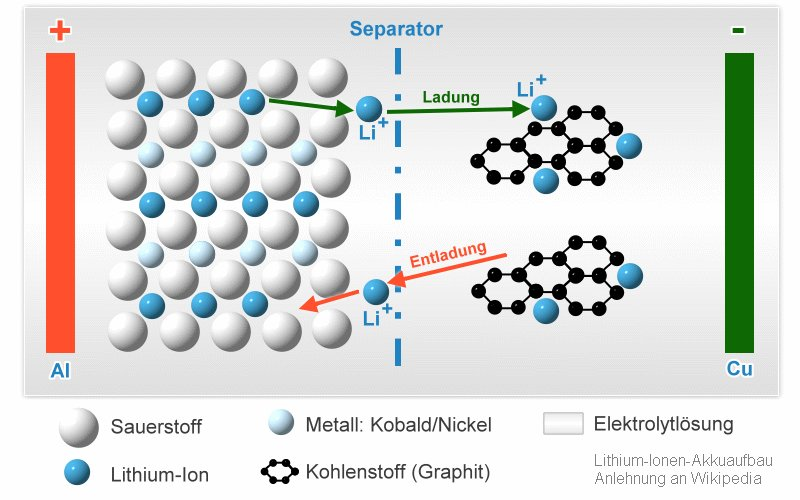
\includegraphics[width=0.74\textwidth]{images/aufbau_liion.jpg}
	\caption{Aufbau/Grundfunktion Lithium-Ionen-Akkumulator \cite{liion_akku_aufbau_funktion1}}
	\label{fig:liion_akku}
\end{figure}

\newpage

\paragraph{Lade-/Entladekurve}
Die typischen Lade-/Entladekurven sind nachfolgend in Abbildungen \ref{fig:liion_akku_ladekurve} und \ref{fig:liion_akku_entladekurve} aufgeführt:

\begin{figure}[h!]
	\centering
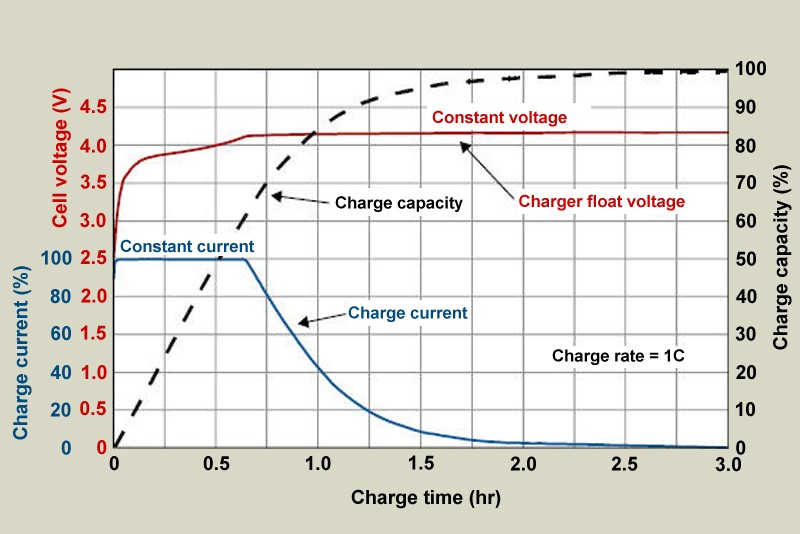
\includegraphics[width=1.0\textwidth]{images/liion_ladekurve.jpg}
	\caption{Ladekurve Lithium-Ionen-Akkumulator \cite{liion_ladekurve}}
\label{fig:liion_akku_ladekurve}
\end{figure}

\begin{figure}[h!]
	\centering
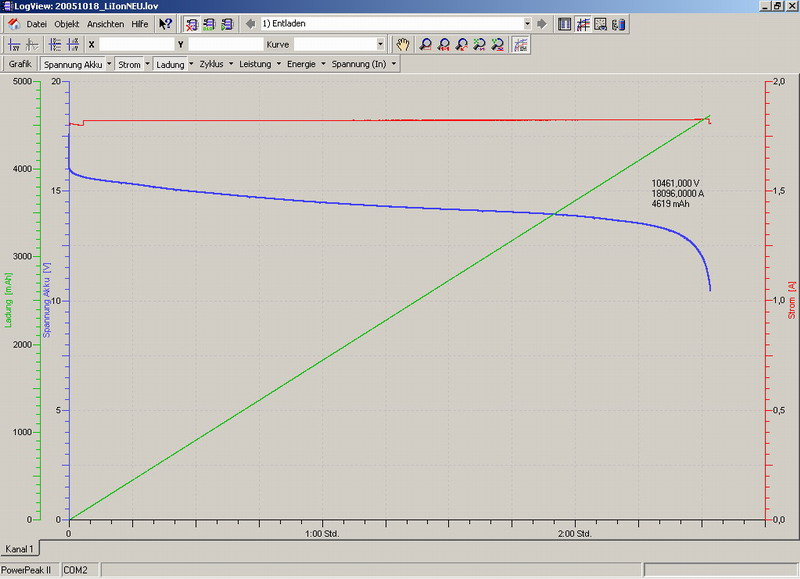
\includegraphics[width=1.0\textwidth]{images/liion_entladekurve.jpg}
	\caption{Entladekurve Lithium-Ionen-Akkumulator \cite{liion_entladekurve}}
\label{fig:liion_akku_entladekurve}
\end{figure}

\newpage

Beim Ladevorgang gemäss Abbildung \ref{fig:liion_akku_ladekurve} ist zu sehen, dass die Batteriespannung innert kurzer Zeit stark ansteigt. Anschliessend ist die Steigung flacher jedoch einigermassen linear. Am Ende wird der Ladestrom reduziert, wobei die Spannung konstant bleibt, bis 100\% der Kapazität erreicht wird.
Nahezu identisch funktioniert der Entladevorgang gemäss Abbildung \ref{fig:liion_akku_entladekurve} jedoch einfach umgekehrt. Die Spannung ist über einen weiten Zeitraum linear und erst am Ende bricht sie zusammen. Eine ähnliche jedoch gespiegelte Kurve kann beim Entladevorgang beobachtet werden.
Zu erwähnen ist noch, dass es sich bei den beiden Figuren in den Abbildungen \ref{fig:liion_akku_ladekurve} und \ref{fig:liion_akku_entladekurve} um unterschiedliche Verschaltungen der Batterien handelt und somit auch um unterschiedliche Ladebereiche. Aus diesem Grund sind auch die Spannungen unterschiedlich, jedoch bleibt die Form der Kurven gleich. Diese Kurve hat somit zwei Stufen: Zuerst wird der Strom begrenzt, damit die thermische Belastung verhindert wird. Danach wird die Spannung begrenzt, damit diese nicht weiter steigt und die Batterien zerstören könnte. Beim Laden wird sie nach oben begrenzt, da sich der Akku sonst aufbläht. Beim Entladen wird die Spannung nach unten begrenzt, da sonst Tiefentladung entstehen könnte. Wobei der Strom immer durch die Anwendung begrenzt werden sollte, da der Innenwiderstand sehr klein ist.

\newpage

\subsection{Vergleich Blei / Lithium-Ionen} \label{kap:Vergleich_liion_pb}

Um die Unterschiede von Lithium-Ionen zu Blei-Akkus besser zu verstehen, sind nachfolgend kurz einige Vor- und Nachteile aufgelistet. Zusätzlich sind in Tabelle \ref{tab:Vergleich} einige Vergleiche dargestellt.

\paragraph{Vorteil Blei}

Kurzfristige Lieferung von hohen Strömen ist für Blei-Akkumulatoren kein Problem. Sie besitzen ein gutes Preis-/Leistungsverhältnis und sind sehr zuverlässig, wenn Wartung und Pflege eingehalten werden. Ebenfalls sind sie relativ einfach in der Ladetechnik.

\paragraph{Nachteil Blei}

Die Energiedichte ist sehr gering. Das heisst, es braucht ein grosses Volumen und somit ein hohes Gewicht, um überhaupt ansatzweise eine gute Kapazität zu erreichen. Auch ist das Elektrolyt säurehaltig, womit Verätzungsgefahr besteht. Zusätzlich können normale Blei-Akkus nur waagerecht gelagert oder verbaut werden, da sonst das schädliche Elektrolyt auslaufen würde.

\paragraph{Vorteil Lithium-Ionen}

Der Akku besitzt eine sehr hohe Energiedichte, was auch für das geringe Gewicht der Akkumulatoren verantwortlich ist. Ebenfalls sind die Akkumulatoren sehr lange haltbar und müssen selten ausgetauscht werden. Auch ist es möglich diese über Monate aufzubewahren, ohne grosse Einbussen in der Ladung zu bemerken.

\paragraph{Nachteil Lithium-Ionen}

Eine aufwändige Ladetechnik und ein Batteriemanagementsystem, kurz BMS, wird benötigt, da die Batterien sehr heikel gegenüber Über- und Unterspannung und auch Übertemperatur reagieren. Somit kommen zusätzliche Kosten hinzu.

\paragraph{Lade-/Entladekurven}

Beide Kurven (siehe Abbildungen \ref{fig:pb_akku_kurve} und \ref{fig:liion_akku_ladekurve}/\ref{fig:liion_akku_entladekurve}) weisen sowohl Gemeinsamkeiten als auch Unterschiede auf. Beide Akkus werden mit dem CCCV (Constant-Current / Constant-Voltage)-Verfahren  geladen. Das bedeutet beim Laden konstanter Strom, bis ein kritischer Punkt in der Spannung erreicht wird. Dann wird die Spannung konstant gehalten um den Strom zu reduzieren. Das Gleiche passiert beim Entladevorgang, einfach umgekehrt. Zu erwähnen ist, dass Lithium-Ionen hier extrem empfindlich sind, wobei mit Blei-Akkus ein wenig gespielt werden kann, ohne dass diese zerstört werden.

\newpage

\begin{table}[h!]
\centering
\begin{tabular}{|l|l|l|}
\hline
\textbf{Akkutyp}                  & \textbf{Bleiakku}                                                                  & \textbf{Lithium-Ionen-Akku}                                                                   \\ \hline
Energiedichte in Wh/kg   & 30-40                                                                     & 70-200                                                                        \\ \hline
(Nenn) Zellspannung      & 2.0 V                                                                     & 3.7 V                                                                         \\ \hline
Ladewirkungsgrad         & 80-85\%                                                                   & 90-95\%                                                                       \\ \hline
Lebensdauer des Akkus    & \begin{tabular}[c]{@{}l@{}}5-15 Jahre\\ \textless3000 Zyklen\end{tabular} & \begin{tabular}[c]{@{}l@{}}15-25 Jahre\\ \textgreater5000 Zyklen\end{tabular} \\ \hline
Selbstentladung im Monat & 5-10\%                                                                    & 1-2\%                                                                         \\ \hline
Preis in Fr/kWh          & 500                                                                       & 800                                                                           \\ \hline
Temperaturbereich ideal  & 15-40$^\circ$C                                                            & 10-40$^\circ$C                                                                \\ \hline
\end{tabular}
\caption{Vergleichswerte Blei - Lithium-Ionen \cite{vergleich_liion_pb}}
\label{tab:Vergleich}
\end{table}

\paragraph{Fazit}

Beide Akkutypen haben ihre Vor- und Nachteile und es kommt stark auf die Anwendung der Batterie an. Für Starterbatterien in einem normalen Auto kann ohne Probleme eine günstige Blei-Batterie verwendet werden, da diese ohne Probleme kurzzeitig einen hohen Startstrom liefern kann. Wenn jedoch wie in unserem Fall ein Fahrzeug dauerhaft mit Akkumulatoren läuft, ist es sinnvoll auf das Gewicht bzw. Lebensdauer und nicht auf den Preis zu achten und somit sind Lithium-Ionen-Batterien hier definitiv die bessere Wahl.
\subsection{Aufbau der Batterie mit Schutzschaltung}
Die beiden originalen Bleibatterien des Detroits hatten einen Nennspannung von $42$ V, was 21 in Serie geschalteten Zellen entspricht. Diese Spannung sollte mit den Lithium Akkus grob erreicht werden, wobei eine Abweichung von $\pm 10$ \% vertreten werden kann. Im Idealfall wäre es dabei möglich, die Zellen in den bereits bestehenden Viererrahmen mit einer Nennspannung von $4\cdot 3.7$ V$=14.8$ V zu belassen.

Mit drei in Serie geschalteten Viererrahmen ergibt sich eine Spannung von $3\cdot 4\cdot 3.7$ V$=44.8$ V, was die Bedingung sehr gut erfüllt. Somit können sämtliche Zellen in den Viererrahmen belassen werden, sodass im Folgenden nur noch die Viererrahmen behandelt werden. Zuerst soll aber Tabelle \ref{tab:bat_vergl} einen Vergleich über die Spannungen der beiden Batterien geben:

\begin{table}[h]
\centering
\begin{tabular}{|l|l|l|}
\hline
\textbf{Batterietyp}              & \textbf{Bleiakkumulator} & \textbf{Lithium-Ionen-Akkumulator} \\ \hline
\textbf{Nennspannung Einzelzelle} & $2.0$ V                            & $3.7$ V                                    \\ \hline
\textbf{Anzahl Serieschaltung}    & 21                                  & 12                                          \\ \hline
\textbf{Minimalspannung Batterie} & $21\cdot1.8$ V$=37.8$ V           & $12\cdot2.8$ V$=33.6$ V                     \\ \hline
\textbf{Nennspannung Batterie}    & $21\cdot2.0$ V$=42.00$ V           & $12\cdot3.7$ V$=44.4$ V                    \\ \hline
\textbf{Maximalspannung Batterie} & $21\cdot2.4$ V$=50.40$ V            & $12\cdot4.1$ V$=49.2$ V                     \\ \hline
\end{tabular}
\caption{Vergleich des originalen Bleiakkumulators mit dem neuen Lithium-Ionen-Akkumulator}
\label{tab:bat_vergl}
\end{table}

Interessanterweise sind sowohl Lade- als auch Entladeschlussspannung der neuen Batterie etwas tiefer als die vergleichbaren Werte des Bleiakkus, obwohl die Nennspannung höher ist. Dies liegt an der wesentlich flacheren Entladekurve des Lithium-Ionen-Akkus im Vergleich zum Bleiakku. Mit diesen Werten kann aber gesagt werden, dass die Spannungen der neuen Batterie sehr gut zu denen des Originals passen.

Insgesamt waren 22 Viererrahmen vorhanden. Mit dem Ziel von zwei Batterien mit je drei Viererrahmen in Serie kann man so pro Batterie eine dreifache Parallelschaltung machen. Dies benötigt insgesamt 18 Viererrahmen, wobei ein Rest von vier übrig bleibt. Der Aufbau der Batterien ist in Abbildung \ref{fig:schema_batterie} gezeigt, wobei jeweils die senkrecht unter einander stehenden Zellen in Serie geschaltet sind:

\begin{figure}[h]
	\centering
	\footnotesize
\begin{tabular}{lp{2mm}lp{2mm}lp{1.5cm}lp{2mm}lp{2mm}l}
\cline{1-1} \cline{3-3} \cline{5-5} \cline{7-7} \cline{9-9} \cline{11-11}
\multicolumn{1}{|l|}{BAT111.1} & \multicolumn{1}{l|}{} & \multicolumn{1}{l|}{BAT121.1} & \multicolumn{1}{l|}{} & \multicolumn{1}{l|}{BAT131.1} & \multicolumn{1}{l|}{} & \multicolumn{1}{l|}{BAT241.1} & \multicolumn{1}{l|}{} & \multicolumn{1}{l|}{BAT251.1} & \multicolumn{1}{l|}{} & \multicolumn{1}{l|}{BAT261.1} \\ \cline{1-1} \cline{3-3} \cline{5-5} \cline{7-7} \cline{9-9} \cline{11-11} 
\multicolumn{1}{|l|}{BAT111.2} & \multicolumn{1}{l|}{} & \multicolumn{1}{l|}{BAT121.2} & \multicolumn{1}{l|}{} & \multicolumn{1}{l|}{BAT131.2} & \multicolumn{1}{l|}{} & \multicolumn{1}{l|}{BAT241.2} & \multicolumn{1}{l|}{} & \multicolumn{1}{l|}{BAT251.2} & \multicolumn{1}{l|}{} & \multicolumn{1}{l|}{BAT261.2} \\ \cline{1-1} \cline{3-3} \cline{5-5} \cline{7-7} \cline{9-9} \cline{11-11} 
\multicolumn{1}{|l|}{BAT111.3} & \multicolumn{1}{l|}{} & \multicolumn{1}{l|}{BAT121.3} & \multicolumn{1}{l|}{} & \multicolumn{1}{l|}{BAT131.3} & \multicolumn{1}{l|}{} & \multicolumn{1}{l|}{BAT241.3} & \multicolumn{1}{l|}{} & \multicolumn{1}{l|}{BAT251.3} & \multicolumn{1}{l|}{} & \multicolumn{1}{l|}{BAT261.3} \\ \cline{1-1} \cline{3-3} \cline{5-5} \cline{7-7} \cline{9-9} \cline{11-11} 
\multicolumn{1}{|l|}{BAT111.4} & \multicolumn{1}{l|}{} & \multicolumn{1}{l|}{BAT121.4} & \multicolumn{1}{l|}{} & \multicolumn{1}{l|}{BAT131.4} & \multicolumn{1}{l|}{} & \multicolumn{1}{l|}{BAT241.4} & \multicolumn{1}{l|}{} & \multicolumn{1}{l|}{BAT251.4} & \multicolumn{1}{l|}{} & \multicolumn{1}{l|}{BAT261.4} \\ \cline{1-1} \cline{3-3} \cline{5-5} \cline{7-7} \cline{9-9} \cline{11-11} 
                               &                       &                               &                       &                               &                       &                               &                       &                               &                       &                               \\ \cline{1-1} \cline{3-3} \cline{5-5} \cline{7-7} \cline{9-9} \cline{11-11} 
\multicolumn{1}{|l|}{BAT112.1} & \multicolumn{1}{l|}{} & \multicolumn{1}{l|}{BAT122.1} & \multicolumn{1}{l|}{} & \multicolumn{1}{l|}{BAT132.1} & \multicolumn{1}{l|}{} & \multicolumn{1}{l|}{BAT242.1} & \multicolumn{1}{l|}{} & \multicolumn{1}{l|}{BAT252.1} & \multicolumn{1}{l|}{} & \multicolumn{1}{l|}{BAT262.1} \\ \cline{1-1} \cline{3-3} \cline{5-5} \cline{7-7} \cline{9-9} \cline{11-11} 
\multicolumn{1}{|l|}{BAT112.2} & \multicolumn{1}{l|}{} & \multicolumn{1}{l|}{BAT122.2} & \multicolumn{1}{l|}{} & \multicolumn{1}{l|}{BAT132.2} & \multicolumn{1}{l|}{} & \multicolumn{1}{l|}{BAT242.2} & \multicolumn{1}{l|}{} & \multicolumn{1}{l|}{BAT252.2} & \multicolumn{1}{l|}{} & \multicolumn{1}{l|}{BAT262.2} \\ \cline{1-1} \cline{3-3} \cline{5-5} \cline{7-7} \cline{9-9} \cline{11-11} 
\multicolumn{1}{|l|}{BAT112.3} & \multicolumn{1}{l|}{} & \multicolumn{1}{l|}{BAT122.3} & \multicolumn{1}{l|}{} & \multicolumn{1}{l|}{BAT132.3} & \multicolumn{1}{l|}{} & \multicolumn{1}{l|}{BAT242.3} & \multicolumn{1}{l|}{} & \multicolumn{1}{l|}{BAT252.3} & \multicolumn{1}{l|}{} & \multicolumn{1}{l|}{BAT262.3} \\ \cline{1-1} \cline{3-3} \cline{5-5} \cline{7-7} \cline{9-9} \cline{11-11} 
\multicolumn{1}{|l|}{BAT112.4} & \multicolumn{1}{l|}{} & \multicolumn{1}{l|}{BAT122.4} & \multicolumn{1}{l|}{} & \multicolumn{1}{l|}{BAT132.4} & \multicolumn{1}{l|}{} & \multicolumn{1}{l|}{BAT242.4} & \multicolumn{1}{l|}{} & \multicolumn{1}{l|}{BAT252.4} & \multicolumn{1}{l|}{} & \multicolumn{1}{l|}{BAT262.4} \\ \cline{1-1} \cline{3-3} \cline{5-5} \cline{7-7} \cline{9-9} \cline{11-11} 
                               &                       &                               &                       &                               &                       &                               &                       &                               &                       &                               \\ \cline{1-1} \cline{3-3} \cline{5-5} \cline{7-7} \cline{9-9} \cline{11-11} 
\multicolumn{1}{|l|}{BAT113.1} & \multicolumn{1}{l|}{} & \multicolumn{1}{l|}{BAT123.1} & \multicolumn{1}{l|}{} & \multicolumn{1}{l|}{BAT133.1} & \multicolumn{1}{l|}{} & \multicolumn{1}{l|}{BAT243.1} & \multicolumn{1}{l|}{} & \multicolumn{1}{l|}{BAT253.1} & \multicolumn{1}{l|}{} & \multicolumn{1}{l|}{BAT263.1} \\ \cline{1-1} \cline{3-3} \cline{5-5} \cline{7-7} \cline{9-9} \cline{11-11} 
\multicolumn{1}{|l|}{BAT113.2} & \multicolumn{1}{l|}{} & \multicolumn{1}{l|}{BAT123.2} & \multicolumn{1}{l|}{} & \multicolumn{1}{l|}{BAT133.2} & \multicolumn{1}{l|}{} & \multicolumn{1}{l|}{BAT243.2} & \multicolumn{1}{l|}{} & \multicolumn{1}{l|}{BAT253.2} & \multicolumn{1}{l|}{} & \multicolumn{1}{l|}{BAT263.2} \\ \cline{1-1} \cline{3-3} \cline{5-5} \cline{7-7} \cline{9-9} \cline{11-11} 
\multicolumn{1}{|l|}{BAT113.3} & \multicolumn{1}{l|}{} & \multicolumn{1}{l|}{BAT123.3} & \multicolumn{1}{l|}{} & \multicolumn{1}{l|}{BAT133.3} & \multicolumn{1}{l|}{} & \multicolumn{1}{l|}{BAT243.3} & \multicolumn{1}{l|}{} & \multicolumn{1}{l|}{BAT253.3} & \multicolumn{1}{l|}{} & \multicolumn{1}{l|}{BAT263.3} \\ \cline{1-1} \cline{3-3} \cline{5-5} \cline{7-7} \cline{9-9} \cline{11-11} 
\multicolumn{1}{|l|}{BAT113.4} & \multicolumn{1}{l|}{} & \multicolumn{1}{l|}{BAT123.4} & \multicolumn{1}{l|}{} & \multicolumn{1}{l|}{BAT133.4} & \multicolumn{1}{l|}{} & \multicolumn{1}{l|}{BAT243.4} & \multicolumn{1}{l|}{} & \multicolumn{1}{l|}{BAT253.4} & \multicolumn{1}{l|}{} & \multicolumn{1}{l|}{BAT263.4} \\ \cline{1-1} \cline{3-3} \cline{5-5} \cline{7-7} \cline{9-9} \cline{11-11} 
\end{tabular}
	\caption{Verschaltung der Batterien}
	\label{fig:schema_batterie}
\end{figure}

Dabei sind auch die jeweils parallelen Zellen miteinander verbunden, sodass alle Zellen der selben Stufe das selbe Potential besitzen. Damit wird für die gesamte Batterie nur noch ein Batteriemanagementsystem benötigt anstelle von drei. Für ausführlichere Informationen zum Batteriemanagementsystem sei auf das nächste Kapitel verwiesen.

Beide Batterien sind jeweils in einer Metallbox aufgebaut. Ebenfalls in dieser Metallbox sind das Steuergerät des zugehörigen Batteriemanagementsystemes, eine Sicherung sowie eine Diode eingebaut. Die Sicherung, eine eigentlich für das Wechselspannungsnetz gebaute Niederspannungs-Hochleistungssicherung, ist vom Hersteller ebenfalls für Gleichspannung spezifiziert, jedoch mit deutlich geringeren Maximalwerten. Dies wird auch durch \cite{siba} gestützt. Die Ursache des niedrigeren Ausschaltstromes liegt am fehlenden Nulldurchgang des Stromes, bei welchem ein Lichtbogen abreissen kann. Der Lichtbogen muss also durch die Distanz und die Füllung gelöscht werden können. Vorteile dieses Sicherungstyps sind, dass sie einfach entfernt werden kann und damit die Stromzufuhr sauber unterbricht. Ebenfalls sprechen die einfache Beschaffbarkeit und der niedrige Preis von Sicherungen für diesen Typ.

Die Diode dient dazu, Ausgleichsströme bei der parallelen Verschaltung der Batterie zu verhindern. Sie ist so in Serie zur Batterie eingebaut, dass der Strom nur in die Entladerichtung fliessen kann. Somit ist es nicht möglich, dass die Batterie mit höherem Potential die Batterie mit niedrigerem Potential auflädt. Es wird jedoch die Batterie mit höherem Potential zu Beginn stärker belastet, wodurch die Ladungen ebenfalls angeglichen werden. Die Ladegeräte sind noch vor den Dioden angeschlossen, da diese sonst keinen Ladestrom fliessen lassen könnten. Dieser Aufbau ist in Abbildung \ref{fig:versch_bat} ersichtlich: \newpage

\begin{figure}[h!]
	\centering
		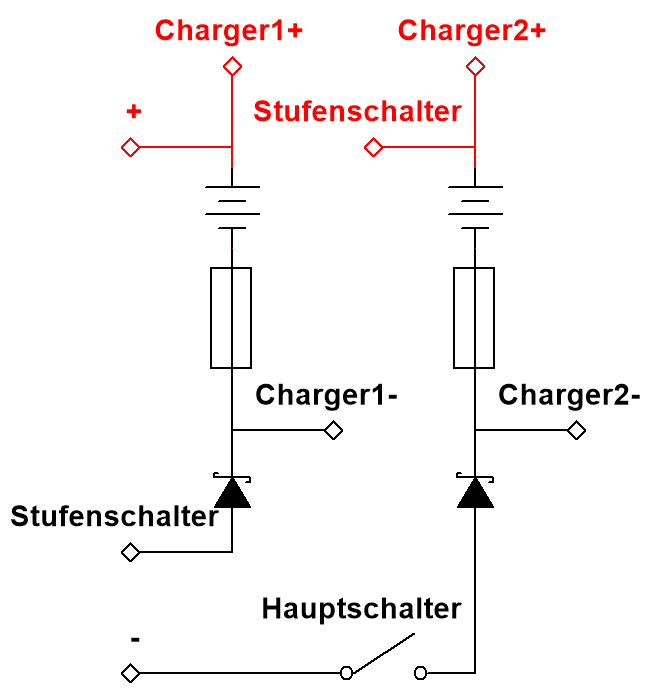
\includegraphics[width=0.45\textwidth]{images/BAT.PNG}
	\caption{Verschaltung der Batterie}
	\label{fig:versch_bat}
\end{figure}

Im Gehäuse eingebaut sind ebenfalls drei Lüfter. Bei hoher Batterietemperatur werden diese vom Batteriemanagementsystem eingeschaltet und sorgen dafür, dass kühle Luft in das Gehäuse eingeblasen wird. Dabei wird die Luft am Diodenkühlkörper vorbei geführt, der zusätzlich über einen eigenen, dauernd eingeschalteten Lüfter verfügt.
\subsection{Das Batteriemanagementsystem}

Als Batteriemanagementsystem (im Folgenden BMS genannt) wird das EMUS BMS des litauischen Herstellers Elektromotus verwendet \cite{emus}. Um dessen Funktion verstehen zu können wird zuerst über den Aufbau und die Funktion berichtet. Anschliessend soll auf die im Programm gesetzten Parameter eingegangen werden. Die Betrachtung erfolgt dabei nur für eine Batterie, wobei die zweite Batterie identisch beschaltet ist. Für ausführlichere Informationen zum BMS sei auf dessen Dokumentation \cite{bms} verwiesen.

\paragraph{Aufbau}
Das eingesetzte Batteriemanagementsystem besteht aus mehreren Teilen: \begin{itemize}
	\item Ein Steuergerät
	\item Ein Zellmodul mit Temperatursensor pro Zelle, insgesamt also 12
	\item Zwei Isolationsadapter zur Kommunikation
	\item Ein Strommessmodul
\end{itemize}

Das \textbf{Steuergerät} ist das Gehirn des BMS. Es verarbeitet sämtliche Informationen der Sensoren und bestimmt damit den Ladezustand der Batterie. Mit diesen Informationen können ebenfalls die Schaltzustände für das Ladegerät sowie für den Hauptschalter bestimmt werden. Ausserdem regelt das Steuergerät die Balancierströme, um sämtliche Zellen auf dem selben Potential zu halten.

Die \textbf{Zellmodule} werden auf jeder Zelle montiert. Sie messen dabei die Spannung und die Temperatur der Einzelzelle. \textcolor{blue}{Bei Bedarf wird ein Balancierstrom durch den Widerstand eingeschaltet}. Die Kommunikation erfolgt dabei seriell durch alle Zellmodul hindurch. Es ist also keine direkte Verbindung vom Zellmodul zum Steuergerät erforderlich.

Die \textbf{Isolationsadapter} sorgen dafür, dass die Signale der Zellmodule galvanisch getrennt an das Steuergerät übertragen werden können. Diese galvanische Trennung sorgt dafür, dass nicht mit hohen Spannungen zum Steuergerät gefahren werden muss und dieses folglich einfacher aufgebaut werden kann. Die galvanische Trennung erfolgt mit Optokopplern.

Das \textbf{Strommessmodul} misst, wie der Name bereits sagt, den Strom. Die Messung erfolgt dabei mittels einem Hallsensor, so dass auch hier ein potentialfreies Signal vorliegt. Die stromführende Leitung wird dabei durch den Sensor geführt, wobei der Hallsensor am Ende das Magnetfeld misst.

\paragraph{Konfiguration}
Das Batteriemanagementsystem muss natürlich auf die verwendete Batterie angepasst werden. Da das BMS frei programmierbar ist, ist es kein Problem, beliebige Einstellungen zu treffen. Einige Parameter sind dabei von der Batterie her gegeben, andere mussten selbst evaluiert werden. Auf einige Parameter soll in diesem Abschnitt eingegangen werden. Sämtliche Parameter sind jedoch im Anhang unter \ref{anh_bms} zu finden. Um die Wiederfindbarkeit zu erleichtern wurden im Anhang die Titel und die Aufteilung von der Bedienungsanleitung des BMS \cite{bms} übernommen. \begin{itemize}
	\item \textit{Max Balancing Stage Duration}: \textcolor{blue}{Im Vergleich zur Zellenkapazität ist der Balancierstrom sehr gering. Um trotzdem eine sauber ausgeglichene Batterie zu haben, wurde dieser Wert sehr hoch gewählt.}
	\item \textit{Allowed Disbalance}: Dieser Wert wurde etwas tiefer als empfohlen angesetzt, wodurch die Zellspannung sehr ähnlich sein sollte.
	\item \textit{Early Balancing Treshold}: Da die Ladekurve über einen langen Bereich sehr flach ist, kann das Balancing bereits am Anfang dieses flachen Bereichs einsetzen, wo Fehler noch deutlicher erkannt werden können. Am Ende der Ladekurve ist diese jedoch wieder steil und Unterschiede fallen deutlich auf.
	\item \textit{Cell Charging Parameter}: Da keine Kommunikation zwischen Ladegerät und BMS stattfindet, wurden diese Werte vom Datenblatt des Ladegerätes übernommen \cite{ladegeraet}.
	\item \textit{Load power reductions}: Da zwischen Antriebsstrang und Batterie keine Kommunikation besteht, wurden sämtliche Funktionen deaktiviert.
\end{itemize}
\subsection{Berechnungen zur Batterie}
Bei der Batterie sind vor allem der maximale Kurzschlussstrom sowie die maximale Verlustleistung von Interesse, da diese für die Sicherung und die Kühlung relevant sind.

Mittels $\frac{dU}{dI}$-Messung konnte der Innenwiderstand der Batterie bestimmt werden. Dabei wurde eine Messung im Leerlauf und eine bei einem Strom von ca. $50$ A durchgeführt, wobei diese Messung für zwölf in Serie geschaltete Zellen ohne Parallelschaltung durchgeführt wurde. Die Messung ergab einen Innenwiderstand von $20$ m$\Omega$ (dies korreliert mit der Herstellerangabe von $1.8$ m$\Omega$ pro Zelle \cite{lev50}), deswegen wird zur Sicherheit mit folgenden Werten gerechnet:
\begin{itemize}
	\item $15$ m$\Omega$ als schlimmster Fall für den Kurzschluss (maximaler Kurzschlussstrom)
	\item $24$ m$\Omega$ als schlimmster Fall für die Verlustleistung (maximale Abwärme)
\end{itemize}

Da jeweils drei Stränge zu 12 Zellen parallel geschaltet sind ergibt sich ein Widerstand von:
\begin{equation*}
	R_B=\frac{1}{\frac{1}{R_1}+\frac{1}{R_2}+\frac{1}{R_3}}=\quad 5\text{ m}\Omega\text{ bzw. } 8\text{ m}\Omega
\end{equation*}

Die Abwärme berechnet sich gemäss der Formel $P=I^2\cdot R$ (für diese Berechnungen wird der Wert von $8$ m$\Omega$ benützt), dies soll zuerst für einen konstanten Ladestrom von $15$ A berechnet werden:
\begin{equation*}
	P_{V,Laden}=\left(15\text{ A}\right)^2\cdot8\text{ m}\Omega=\quad\underline{1.8\text{ W}}
\end{equation*}

Für den maximalen Fahrstrom ergibt sich eine Abwärme von:
\begin{equation*}
	P_{V,Max}=\left(100\text{ A}\right)^2\cdot8\text{ m}\Omega=\quad\underline{80\text{ W}}
\end{equation*}

Bei der Ladung kann die Abwärme der Batterie als irrelevant angesehen werden. Auch bei grosser Belastung entsteht keine grosse Wärme. Trotzdem können durch das Batteriemanagementsystem bei Bedarf Lüfter eingeschaltet werden, um die Batterien zu kühlen. Die sehr geringe Eigenerwärmung der Zellen konnten bei einem Versuch bestätigt werden, bei dem eine Einzelzelle ($3.7$ V, $50$ Ah) ungefähr eine halbe Stunde mit einem Strom von $30$ A belastet wurde und sich nicht fühlbar erwärmte.

Der schlimmste Fall eines Kurzschlusses ist ein Kurzschluss direkt an den Klemmen der Batterie. In diesem Fall wird der Stromfluss nur durch den Innenwiderstand der Batterie beschränkt. Im schlimmsten Fall muss mit der Ladeschlussspannung und einem kleinen Innenwiderstand der Batterie gerechnet werden. Der Kurzschlussstrom berechnet sich gemäss $I=\frac{U}{R}$ zu:
\begin{equation*}
	I_k=\frac{12\cdot 4.2\text{ V}}{5\text{ m}\Omega}=\quad\underline{10\ 800\text{ A}}
\end{equation*}

\subsection{Kapazität der Batterie}\label{sec:ah}
\color{blue}Die Batteriekapazität pro Zelle wird mit $50$ Ah angegeben \cite{lev50}, woraus bei drei parallel geschalteten Zellen eine theoretische Kapazität von $150$ Ah ergibt. Die Messungen über das BMS haben dann aber gezeigt, dass dieser Wert deutlich zu hoch ist, realistischer erscheint ein ungefähr halb so grosser Wert, womit auch der Energiegehalt der Zellen deutlich geringer ausfällt. Um diese Diskrepanz zu erklären, wurde nach Gründen für den doch deutlichen Unterschied gesucht: \begin{itemize}
	\item Die Entladeschlussspannung wurde etwas höher gewählt, wodurch sich nicht die gesamte Kapazität entnehmen lässt.
	\item Die Entladung erfolgte mit einem deutlich höheren Strom als bei der Herstellerangabe, wodurch die Entladeschlussspannung schneller erreicht ist (durch den höheren Spannungsabfall am Innenwiderstand der Batterie).
	\item Die Batterien altern mit der Zeit. Bei der Batterie selbst wurde kein Datum für deren Erstellung gefunden, jedoch deuten andere Bauteile auf eine Produktion Anfang 2011 hin, wodurch ein Alter von sieben Jahren resultiert.
	\item Einige Minuten nach dem Beenden der Entladung steigt die Zellenspannung wieder leicht an.
\end{itemize}

Wird angenommen, dass die etwas schonendere Ladekurve sowie die höhere Stromabnahme die Batteriekapazität um jeweils 10\% des Originalwerts verringern (dies ist eine nicht weiter begründete Schätzung), so entfällt auf die Alterung selbst noch ein Rückgang von 80\% auf 50\%, entsprechend einer Alterung von 37.5\%. Damit kann nun die prozentuale Alterung pro Jahr berechnet werden, Formel \ref{eq:Alterung}:
\begin{equation}
	1-0.375=\left(1-x_A\right)^7\qquad\rightarrow\qquad x_A=\quad\underline{0.0649}
\label{eq:Alterung}
\end{equation}

Die jährliche Alterung erscheint mit 6.5\% pro Jahr durchaus realistisch, wobei auch hier eine grosse Unsicherheit besteht, da die Temperatur einen sehr grossen Einfluss auf die Alterung hat \cite{bat_alterung}.

Als Hauptgründe für die Reduktion der Batteriekapazität können also zum einen eine andere Lastkurve sowie die Alterungsprozesse über sieben Jahre genannt werden.



\color{black}\newpage
\section{Antrieb}

Im \textsc{Detroit} kann die Geschwindigkeit mittels eines Stufenschalters mit fünf Positionen ausgewählt werden. Um die Funktion des Stufenschalters zu verstehen, ist es unabdingbar, zu Beginn einen Blick auf die Funktionsweise des Motors zu richten. Anschliessend werden die verschiedenen Schaltungen, die mit dem Stufenschalter realisierbar sind, vorgestellt.

\subsection{Funktion des Reihenschlussmotores}\label{gm}

Grundsätzlich ist der verwendete Motor ein Gleichstrommotor. Für diesen Motor sind die beiden Gleichungen \ref{eq:motor_dc_i} und \ref{eq:motor_dc_u} ausschlaggebend, welche die Funktion des idealen Ankers beschreiben ($k$ steht dabei für eine Maschinenkonstante, die die Konstruktion des Motors zusammenfasst):
\begin{equation}
	M_{el}=k\cdot\Phi_E\cdot I_A
\label{eq:motor_dc_i}
\end{equation}
\begin{equation}
	\omega_{me}=\frac{U_i}{k\cdot \Phi_E}
\label{eq:motor_dc_u}
\end{equation}
Wichtig ist, dass diese Gleichungen für den idealen Anker gelten. Bei einem realen Motor addiert sich zur induzierten Spannung $U_i$ noch die Spannung über dem ohmschen Ankerwiderstand $R_A\cdot I_A$. Ausserdem entstehen im Motor selbst Reibungen, die das verfügbare mechanische Drehmoment reduzieren (beispielsweise Lager oder Lüfter).

Wird angenommen, dass die Nichtlinearitäten klein sind im Vergleich zum idealen Modell, kann gesagt werden, dass der Strom proportional zum Moment und die Spannung proportional zur Winkelgeschwindigkeit ist. Mit dem Erregerfluss $\Phi_E$ können dabei beide Grössen beeinflusst werden: \begin{itemize}
	\item Bei erhöhtem Erregerfluss wird das Moment pro Strom grösser, jedoch die Winkelgeschwindigkeit pro Spannung kleiner
	\item Bei verringertem Erregerfluss wird die Winkelgeschwindigkeit pro Spannung grösser, jedoch das Moment pro Strom kleiner
\end{itemize}

Über einen veränderlichen Erregerfluss können also gezielt Moment und Geschwindigkeit aneinander angepasst werden. Genau dieses Verhalten wird im Reihenschlussmotor ausgenutzt. Bevor jedoch auf dessen Funktion eingegangen wird, soll der schematische Aufbau des Reihenschlussmotors in Abbildung \ref{fig:reihenschluss} erläutert werden:

\newpage

\begin{figure}[h!]
	\centering
		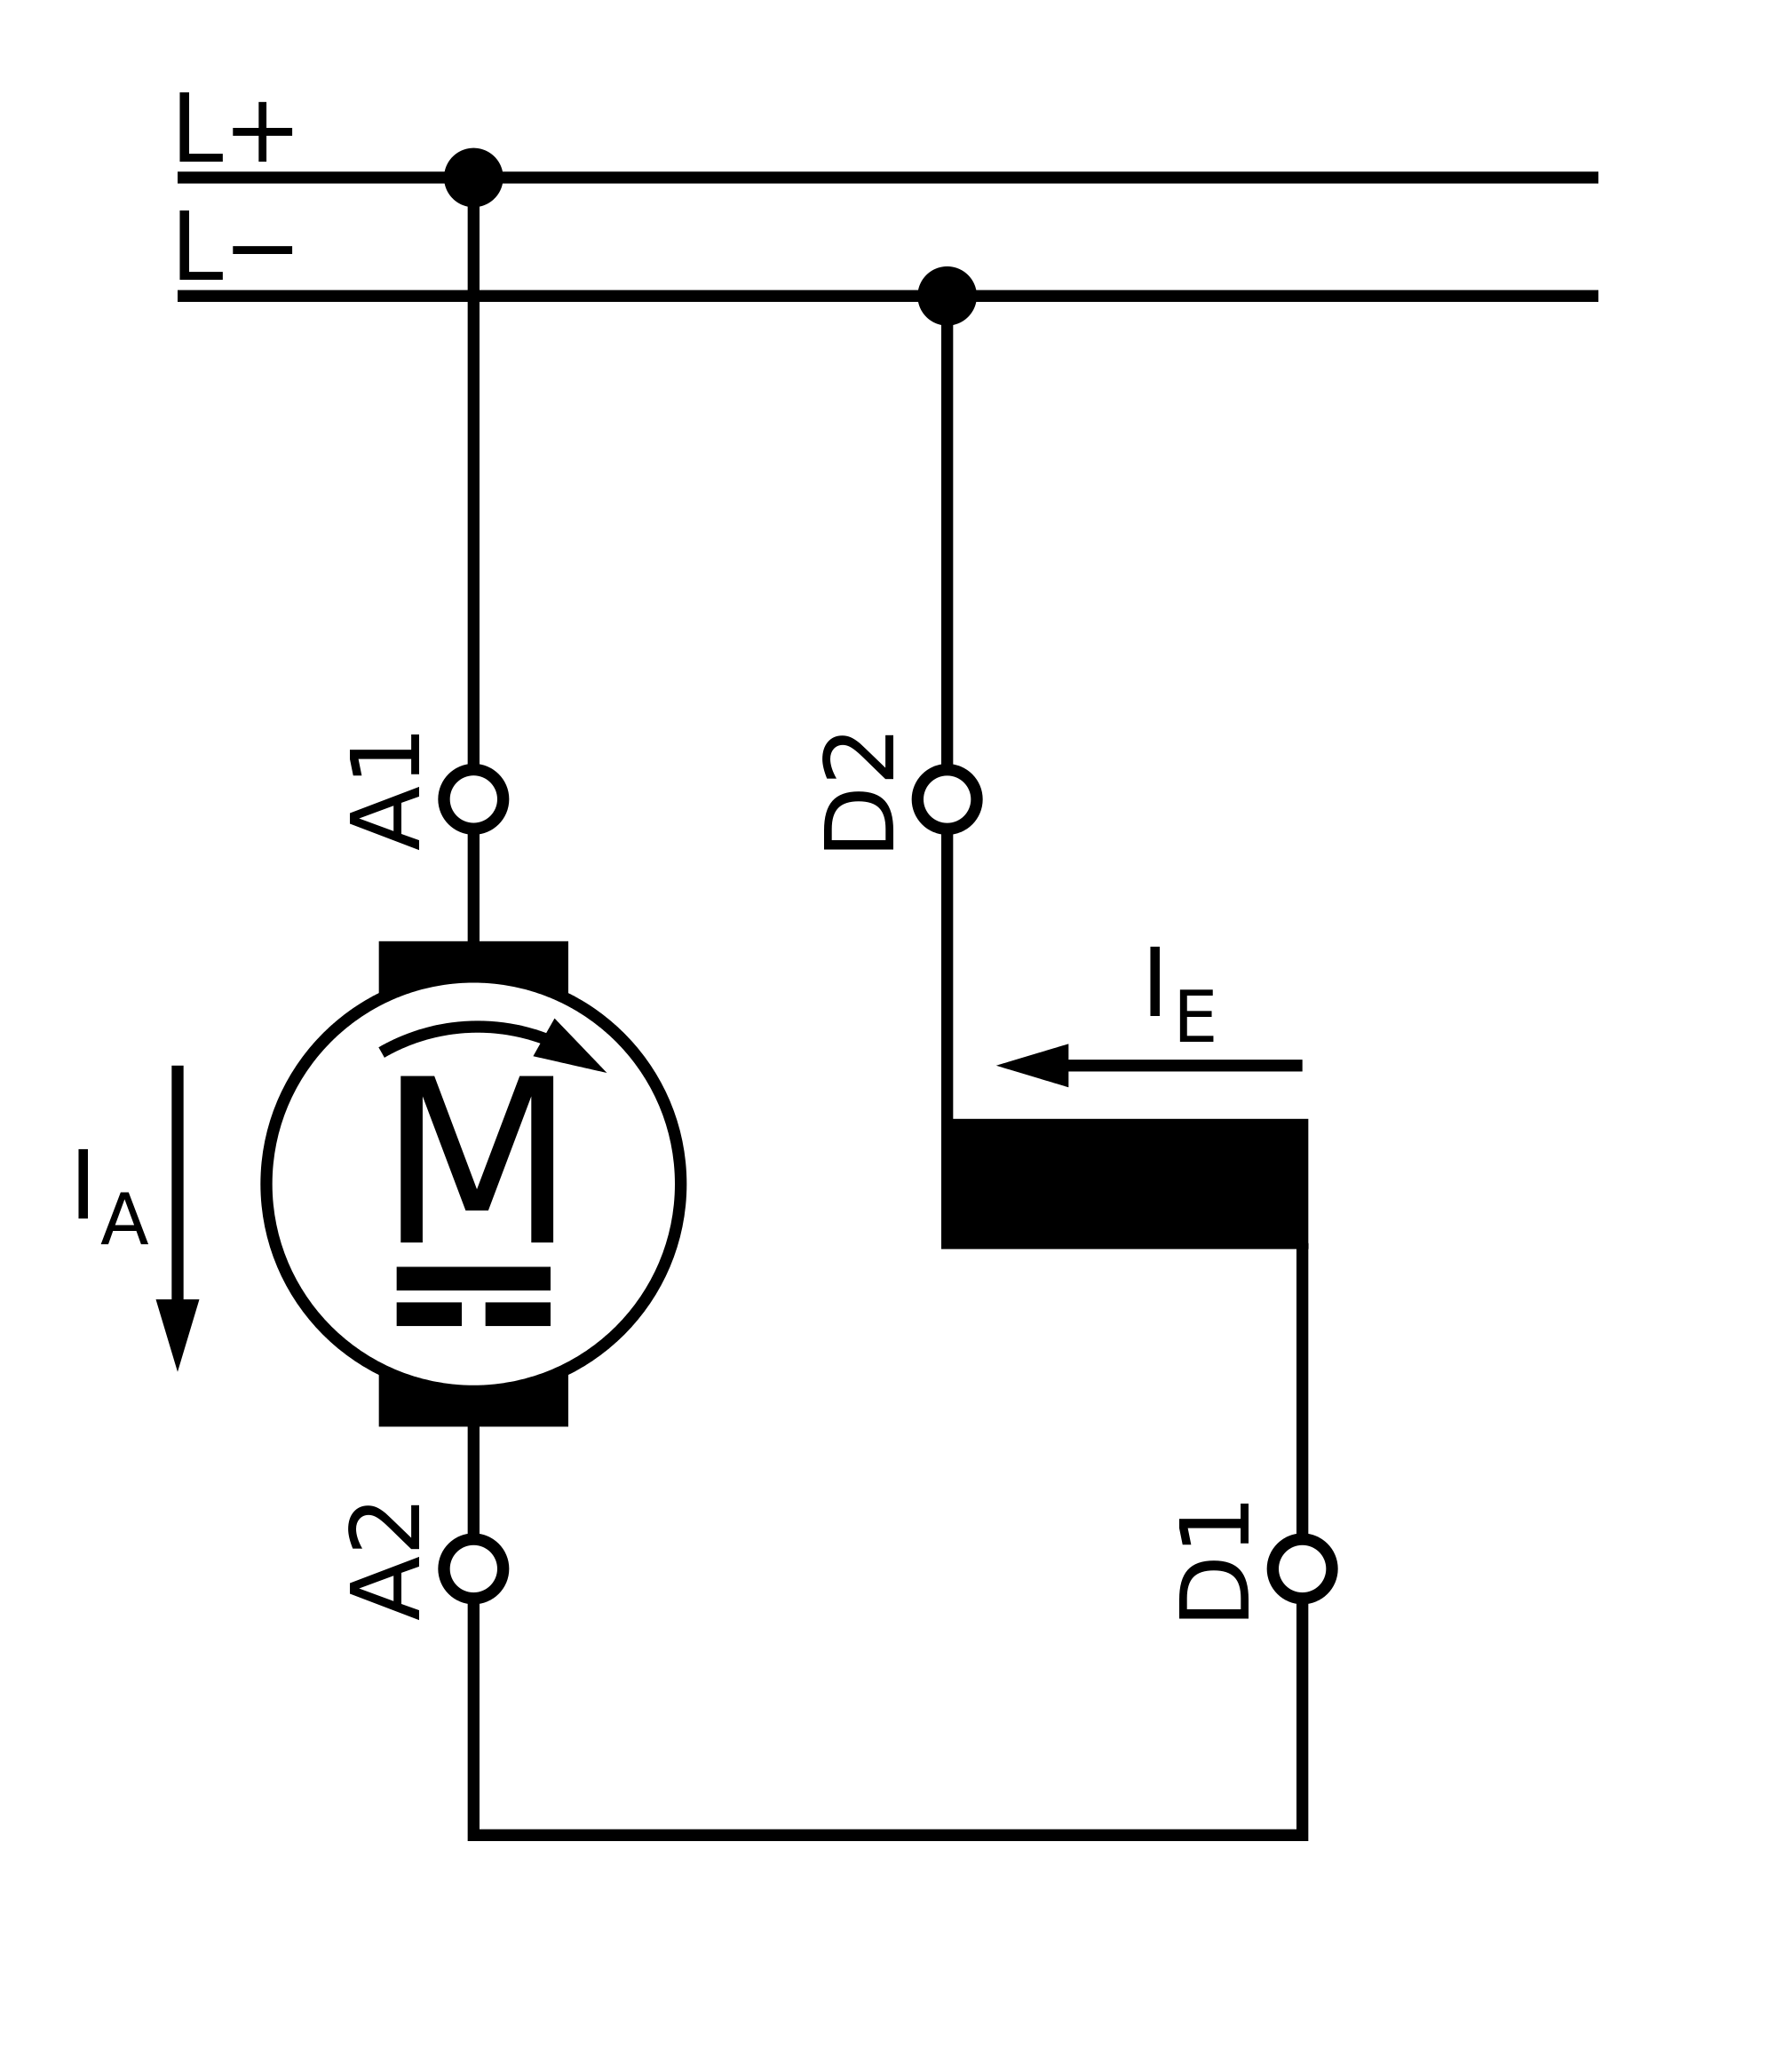
\includegraphics[width=0.45\textwidth]{images/Reihenschlussmotor.png}
	\caption{Elektrisches Schema eines Reihenschlussmotors \cite{wiki_reihenschlussmotor}}
	\label{fig:reihenschluss}
\end{figure}

Der Erregerfluss ist dabei vom Erregerstrom abhängig, wie in Formel \ref{eq:dc_motor_phie} gezeigt ist:
\begin{equation}
	\Phi_E=\frac{L_E}{N_E}\cdot I_E
\label{eq:dc_motor_phie}
\end{equation}

Da durch Anker und Erregerwicklung der selbe Strom fliesst, somit gilt $I_A=I_E$, sieht man sehr gut, dass bei sinkendem Stromfluss zum einen das Moment aufgrund von Formel \ref{eq:motor_dc_i} kleiner wird, zum anderen das Moment auch durch die schwächere Erregung (aufgrund des geringeren Stromes) kleiner wird. Das Moment ist also quadratisch abhängig vom Stromfluss. Wird ausserdem die weitere Maschinenkonstante $c=k\cdot\frac{L_E}{N_E}$ gesetzt, resultieren für die ideale Reihenschlussmaschine die beiden Formeln \ref{eq:reihenschluss_m} und \ref{eq:reihenschluss_w}:
\begin{equation}
	M_{el}=c\cdot I^2
\label{eq:reihenschluss_m}
\end{equation}
\begin{equation}
	\omega_{me}=\frac{U_i}{c\cdot I}
\label{eq:reihenschluss_w}
\end{equation}
Da auch bei der Reihenschlussmaschine der ohmsche Spannungsabfall über Anker- und Erregerwicklung einen zum Strom proportionalen Spannungsabfall bewirkt, stellt sich für jede angelegte Spannung automatisch ein Gleichgewicht zwischen Drehzahl und Drehmoment ein. Dies erlaubt jedoch weder eine vernünftige Regelung der Geschwindigkeit, noch ist es in jedem möglichen Arbeitspunkt besonders effizient.

Um diese Probleme anzugehen, wird mit der sogenannten Feldschwächung gearbeitet: Bei niedrigen Drehzahlen, wo hohes Moment gefordert ist, wird die Erregung komplett in Serie zum Anker geschaltet. Werden bei höheren Drehzahlen nicht mehr so hohe Momente benötigt, wird ein Teil des Stromes "`an der Erregerwicklung vorbei"' 
geleitet, sodass die Erregung zusätzlich geschwächt wird. Dies wird als Feldschwächung bezeichnet.

\subsection{Funktion des Stufenschalters}

Diese Effekte, die beim Reihenschlussmotor bereits vorgestellt wurden, werden vom Stufenschalter gesteuert. Dies ist zum einen die Spannung über dem Motor, zum anderen ist auch eine Feldschwächung möglich. Im Folgenden sollen die fünf Fahrstufen sowie die ursprüngliche Ladestufe vorgestellt werden.

\begin{minipage}{0.49\textwidth}
	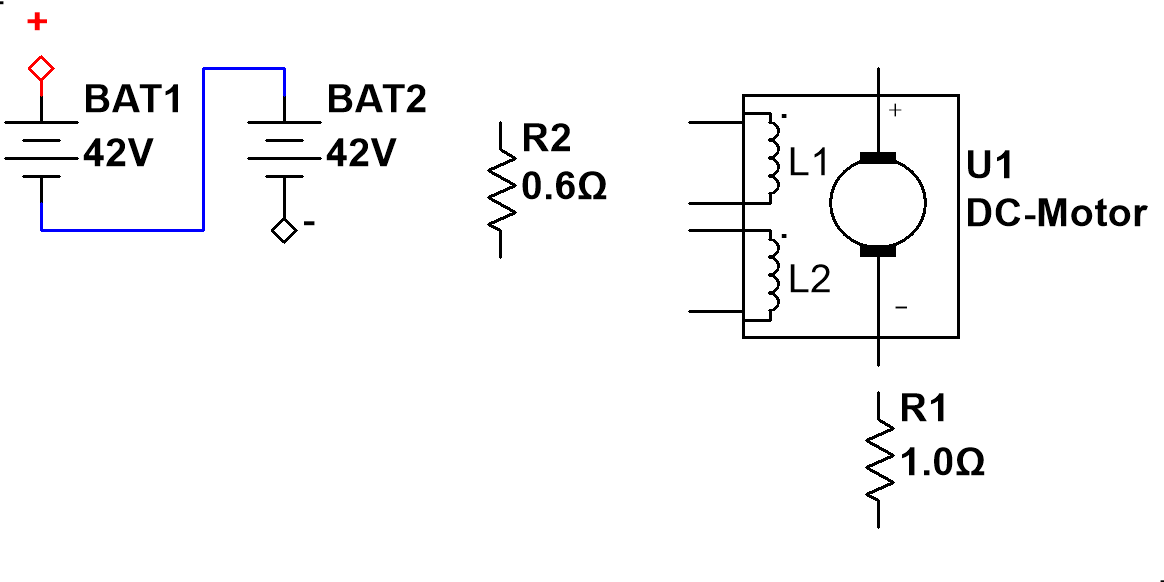
\includegraphics[width=\columnwidth]{images/Stufenschalter/Laden.png}%
\end{minipage}
\begin{minipage}{0.5\textwidth}
	\paragraph{Stufe: Laden}
	In der Nullstellung des Stufenschalters ist die Batterie im Lademodus. Dazu sind beide Batterien in Serie geschalten, sodass beide Batterien mit dem selben Strom geladen werden. Sämtliche Komponenten des Motors sowie die beiden Widerstände sind nicht angeschlossen. Diese Stufe ist auch nach dem Umbau des \textsc{Detroits} weiterhin vorhanden. Das serielle Laden der beiden Batterien wird aber durch die verbauten Dioden verhindert.
\end{minipage}

\begin{minipage}{0.49\textwidth}
	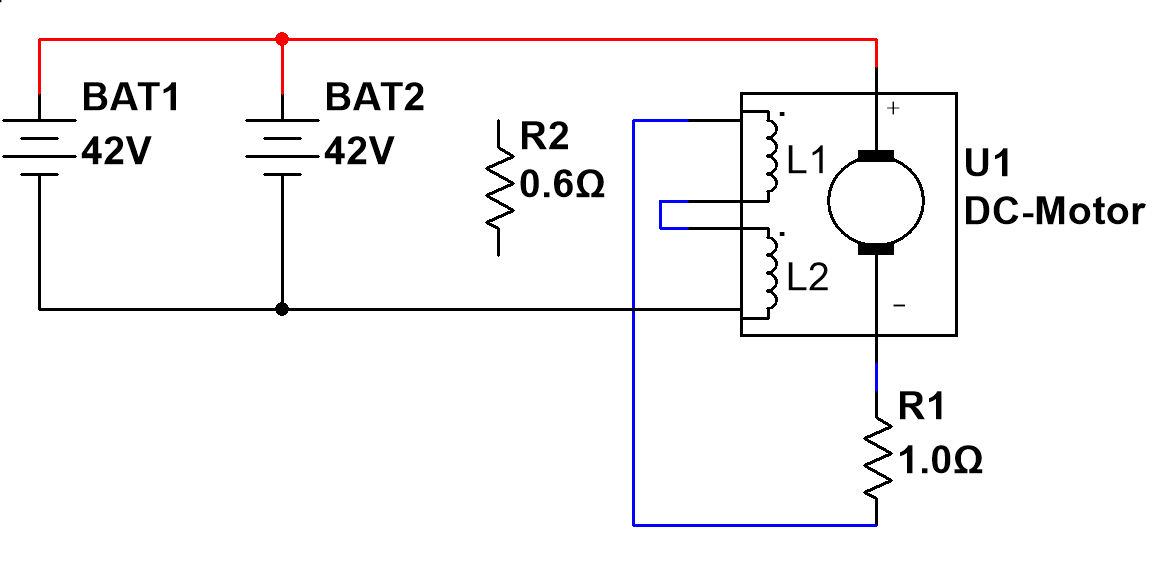
\includegraphics[width=\columnwidth]{images/Stufenschalter/Stufe_1.png}%
\end{minipage}
\begin{minipage}{0.5\textwidth}
	\paragraph{Stufe: Eins}
	In der ersten Fahrstufe werden die beiden Batterien parallel geschaltet, wodurch zum einen die Spannung verringert wird, zum anderen auch der für grosse Momente benötigte Strom geliefert werden kann. Um ein maximales Moment zu erreichen, sind beide Feldwicklungen in Serie angeschlossen, was bewirkt dass durch beide der volle Fahrstrom fliesst. Ausserdem ist zur Begrenzung des Anlaufstromes (da im ersten Moment die induzierte Spannung $U_i=0V$ beträgt) der Widerstand $R_1$ in Serie geschaltet.
\end{minipage}

\begin{minipage}{0.49\textwidth}
	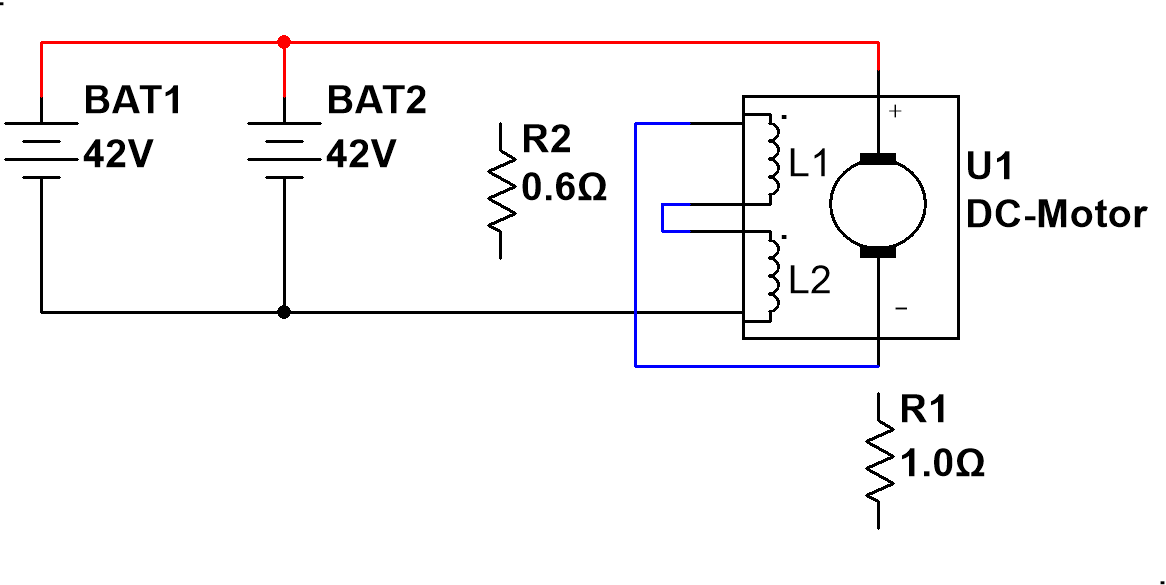
\includegraphics[width=\columnwidth]{images/Stufenschalter/Stufe_2.png}%
\end{minipage}
\begin{minipage}{0.5\textwidth}
	\paragraph{Stufe: Zwei}
	Die zweite Stufe ist fast gleich aufgebaut wie die erste. Auch hier werden für ein möglichst grosses Moment die Serieschaltung der Erregerwicklungen sowie die Parallelschaltung der Batterien verwendet. Der einzige Unterschied zur ersten Fahrstufe ist, dass der Anfahrwiderstand $R_1$ überbrückt und somit funktionslos ist. Durch den weggefallenen Spannungsabfall über dem Anfahrwiderstand wird die erreichbare induzierte Spannung grösser, ohne dabei das erreichbare Moment zu reduzieren.
\end{minipage}

\begin{minipage}{0.49\textwidth}
	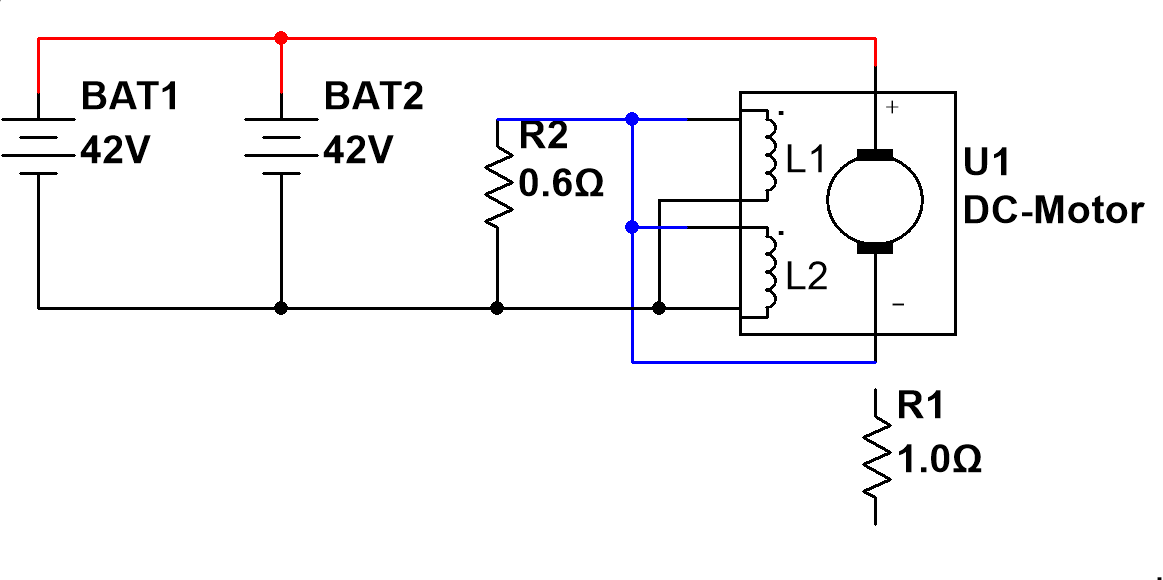
\includegraphics[width=\columnwidth]{images/Stufenschalter/Stufe_3.png}%
\end{minipage}
\begin{minipage}{0.5\textwidth}
	\paragraph{Stufe: Drei}
	In der dritten Stufe wird von der Feldschwächung Gebrauch gemacht. Die beiden Erregerwicklungen sind nicht mehr seriell, sondern parallel geschaltet. Ausserdem ist der Widerstand $R_2$ parallel zu den beiden Erregerwicklungen geschaltet. Durch diese Parallelschaltung ist der Stromfluss in der Erregerwicklung und damit die Erregung selbst deutlich kleiner als in den vorherigen Fahrstufen, wodurch eine höhere Winkelgeschwindigkeit bei reduziertem Moment ermöglicht wird. Die beiden Batterien sind weiterhin parallel geschaltet.
\end{minipage}

\begin{minipage}{0.49\textwidth}
	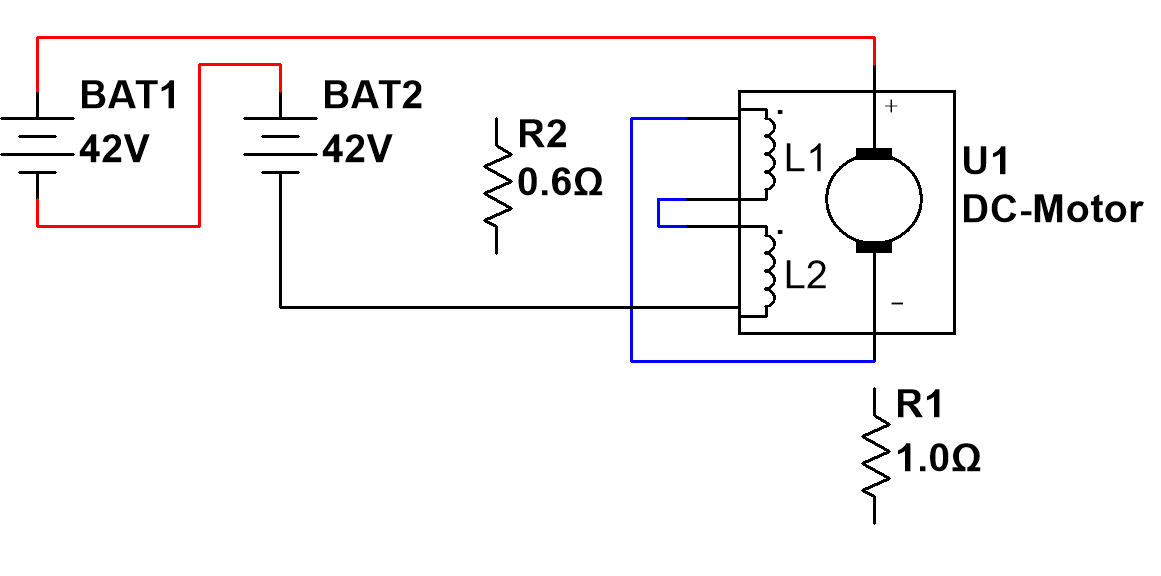
\includegraphics[width=\columnwidth]{images/Stufenschalter/Stufe_4.png}%
\end{minipage}
\begin{minipage}{0.5\textwidth}
	\paragraph{Stufe: Vier}
	In der vierten Fahrstufe wird die Spannung durch Serieschaltung der Batterien erhöht. Um weiterhin grosse Kräfte zu ermöglichen, wird die Erregerwicklung wieder von parallel nach seriell verschaltet, wodurch keine Feldschwächung entsteht. Stufe vier ist deswegen sehr ähnlich aufgebaut wie Stufe zwei, jedoch sind aufgrund der verdoppelten Spannung höhere Leistungen erzielbar als in Stufe zwei. Es ist gut möglich, dass bei den ursprünglichen Blei-Batterien dieser Leistungszuwachs bei hohen Strömen durch den Innenwiderstand der Batterien zum Teil wieder ausgeglichen wurde. Bei den modernen Lithium-Ionen-Akkumulatoren kann dies jedoch dementiert werden. Es ist zudem aufgrund der hohen Spannung und des gleichzeitig starken Feldes zu vermuten, dass in dieser Stufe die grössten Momente entwickelt werden konnten. Dies entspricht einer Überlast und wird durch den Überstromschutz der Batterien verhindert.
\end{minipage}

\begin{minipage}{0.49\textwidth}
	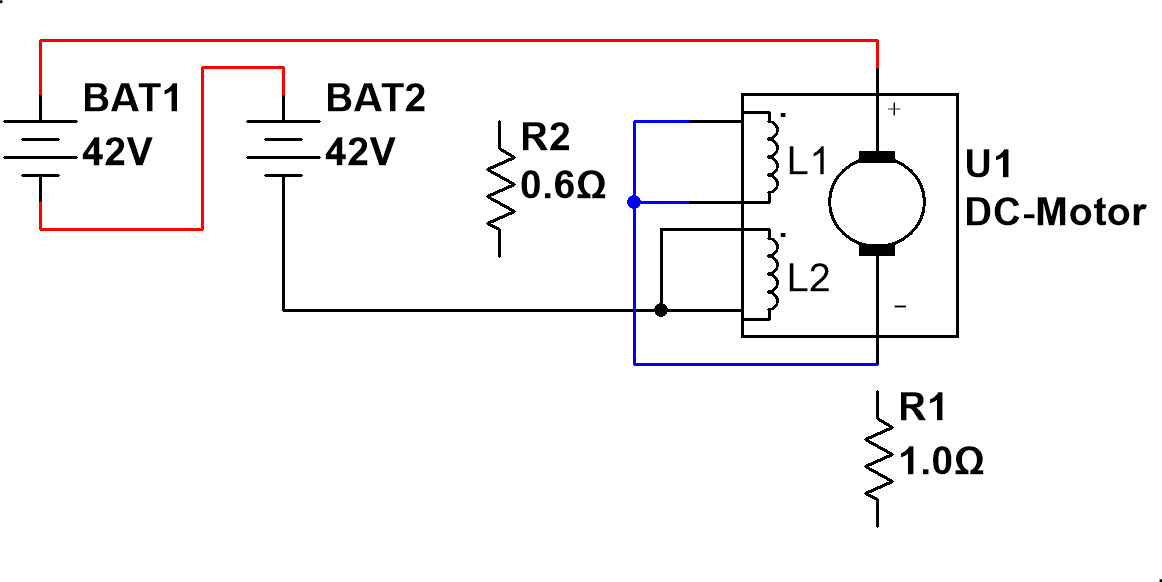
\includegraphics[width=\columnwidth]{images/Stufenschalter/Stufe_5.png}%
\end{minipage}
\begin{minipage}{0.5\textwidth}
	\paragraph{Stufe: Fünf}
	Auch in der fünften und damit höchsten Fahrstufe sind die beiden Batterien für eine höhere Spannung in Serie geschaltet. Hier wird erneut die Feldschwächung angewendet, indem die beiden Erregerwicklungen parallel geschalten werden und damit der Fluss reduziert wird. Im Gegensatz zur Stufe drei, bei welcher die Erregerwicklungen ebenfalls parallel geschaltet werden, wird hier auf die zusätzliche Parallelschaltung des Widerstandes $R_2$ und damit auf die weitere Reduktion des Feldes verzichtet. Dadurch sollten sich auch noch bei hohen Geschwindigkeiten genügende Momente ergeben.
\end{minipage}

Die Fahrstufen werden dabei vom Stufenschalter mechanisch geschaltet, indem unter den Kontaktfingern mittels Kupferplatten Kontakte verbunden (und damit beispielsweise Widerstände überbrückt) werden. Die Lagen dieser Kupferplatten sind im Originalschema zu finden, wie es im Anhang unter \ref{schema_original} aufgezeigt ist. Ausserdem ist ein Blick in das Innere des Stufenschalters in Abbildung \ref{fig:Stufenschalter} gegeben:

\begin{figure}[h]
	\centering
		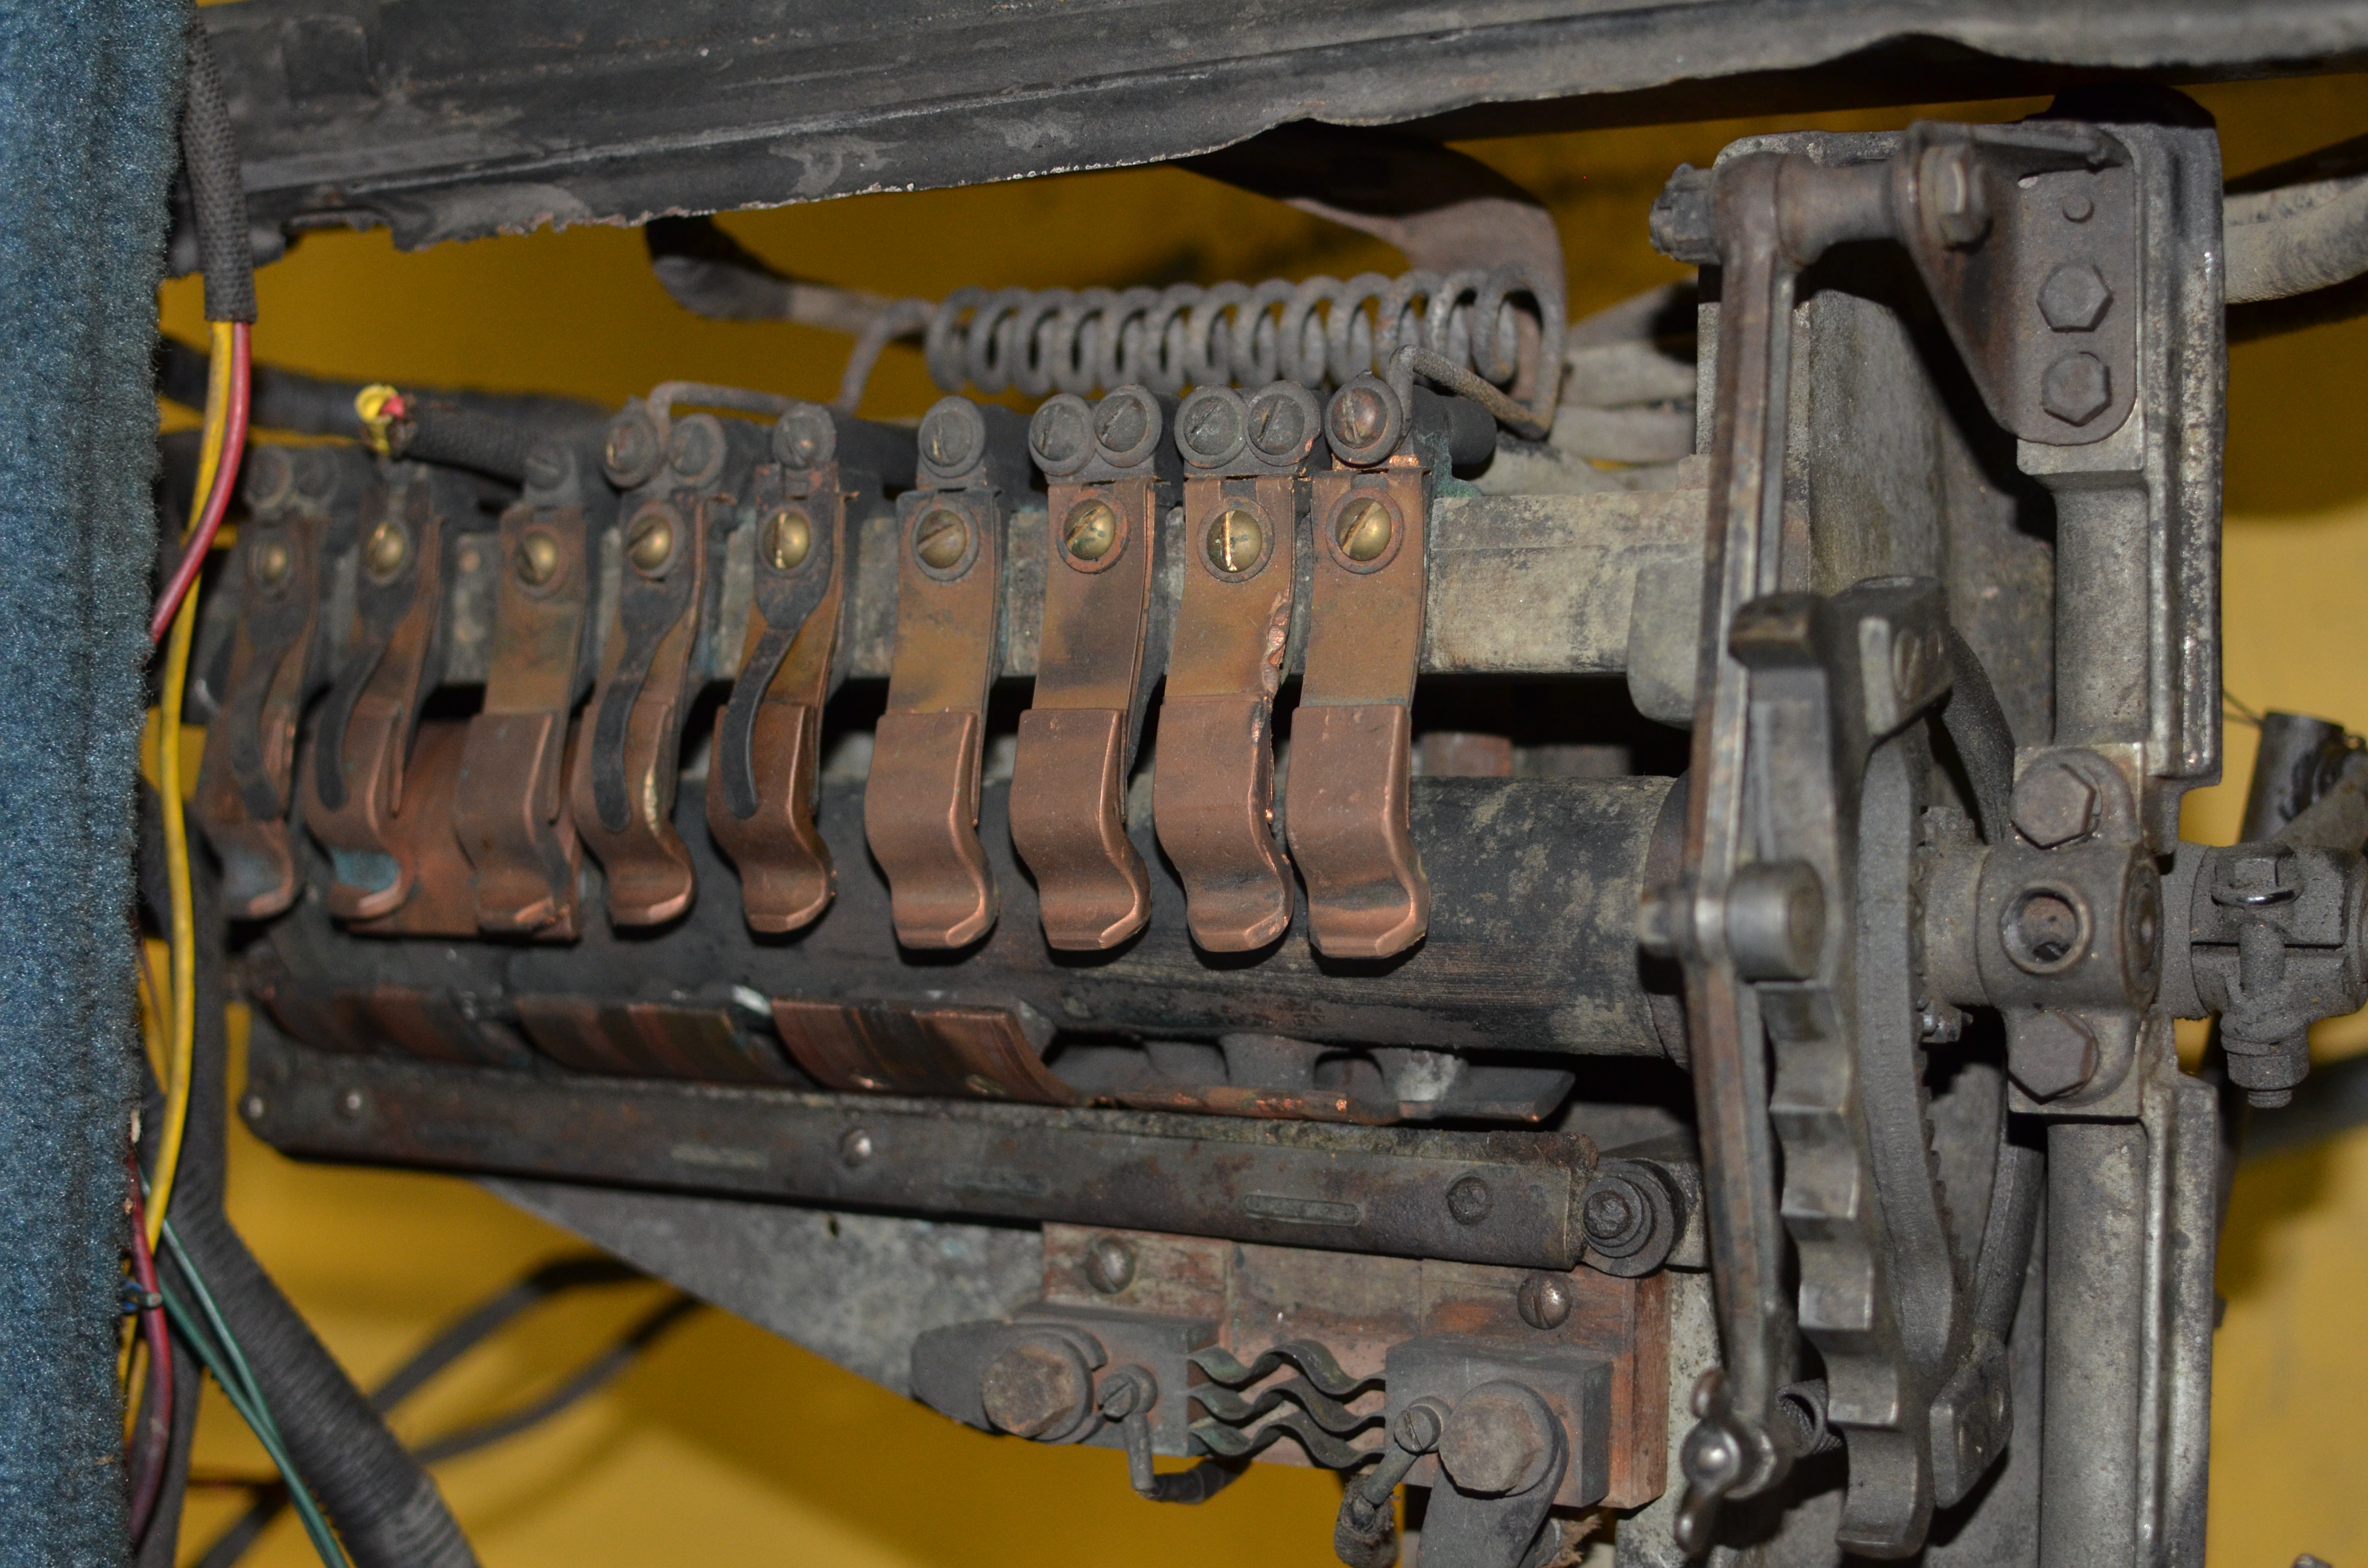
\includegraphics[width=0.8\textwidth]{images/Stufenschalter/Foto}
	\caption{Blick in den geöffneten Stufenschalter}
	\label{fig:Stufenschalter}
\end{figure}

Glücklicherweise befand sich der Stufenschalter in einem guten Zustand, sodass lediglich etwas Staub entfernt werden musste. Ausserdem wurde ein Teil der Verkabelung erneuert, sodass diese ebenfalls am Stufenschalter befestigt werden konnte.

\newpage
\section{Hilfsstromversorgung}
Mit der Hilfsstromversorgung sind sämtliche Komponenten gemeint, die nicht direkt zum Antrieb gehören. Diese Bauteile laufen mit einer Spannung von $12$ VDC, welche von einem Spannungswandler aus einer Batterie gewonnen wird. Dabei wird eine leichte Asymmetrie der Batterien toleriert, da diese beim Parallelschalten durch den Stufenschalter ausgeglichen werden (durch die stärkere Belastung der volleren Batterie).

\subsection{Steuerplatine}
Um die Kommunikation zu und von den beiden Steuerplatinen zu implementieren, wurde eine sogenannte Steuerplatine erstellt. Diese regelt sämtliche Funktionen, welche mit dem BMS zu tun haben. Das Schema dieser Steuerplatine ist im Anhang unter \ref{Anh_Steuerplatine} zu finden. Dort sind einzelne Bereiche eingefärbt, auf welche im Folgenden eingegangen werden soll.

\paragraph{Gelb: Anschlüsse}
Die gelb hinterlegten Komponenten bilden die Verbindung zu den weiteren Komponenten. Mit Ausnahme der $12$ V-Zuleitung wurden sämtliche Verbindungen als Schraubklemmen ausgeführt. Lediglich letztere wurde aufgrund des grossen Stromes und der benachbarten Montage direkt aufgelötet. Die einzelnen Verbindungen erfüllen folgende Aufgaben: \begin{itemize}
	\item \textbf{BMS1 / BMS2}: Verbindung zum ersten und zweiten Batteriemanagementsystem
	\item \textbf{12Fahren}: Die $12$ V-Spannungsversorgung, wenn das Fahrzeug eingeschaltet ist
	\item \textbf{Voltmeter}: Verbindung zur Batteriestandanzeige
	\item \textbf{Hauptschalter}: Verbindung zu den Spulenkontakten des Hauptschalters
	\item \textbf{230}: Verbindung zum $230$ VAC-Eingang, sowie den beiden Ladegeräten
	\item \textbf{Luefter1 / Luefter2}: Verbindung zu den beiden Batteriekühlern
\end{itemize}

\paragraph{Rot: Spannungsversorgung}
Die Spannungsversorgung regelt, wie der Name bereits andeutet, die Versorgung der Steuerung mit Spannung. Dabei sind die beiden Fälle für das eingeschaltete Fahrzeug (Zustand "Fahren") sowie für den Zustand "Laden" zu unterscheiden.

Beim Zustand \textbf{Fahren} wird die gesamte Steuerung über den im Fahrzeug eingebauten DC-DC-Wandler versorgt, der ausserdem die Beleuchtung mit Spannung beliefert. In diesem Zustand sind sämtliche Funktionen verfügbar. Ausserdem werden die $24$ V des BMS durch die Diode $D_1$ und den Spannungswander $U_3$ bereitgestellt. Die Dioden sorgen dabei für die Trennung der beiden Spannungswandler.

Beim \textbf{Laden} ist es wichtig, dass das Fahrzeug nicht eingeschaltet werden kann. Damit wird verhindert, dass versehentlich mit dem noch eingesteckten Fahrzeug losgefahren wird. Dies wird dadurch sichergestellt, dass das Relais $U_4$ beim Anschluss von $230$ VAC automatisch die Spannungszufuhr für die Steuerung unterbricht. Da jedoch auch beim Laden das BMS eingeschaltet sein soll, wird dieses über einen Spannungswandler vom $230$ VAC-Netz versorgt.

\paragraph{Grau: Passive Signale}
Die beiden passiven Signale umfassen die Information, dass das System eingeschaltet ist beziehungsweise am $230$ VAC-Netz angeschlossen ist. Dies sind logische 0-(entspricht $<1$ V) und 1-(entspricht $>4$ V) Signale. Da bei beiden Zuständen jeweils eine eigene $12$ V Versorgungsspannung benötigt wird, können die benötigten Signale einfach mittels passivem Spannungsteiler aus diesen Versorgungsspannungen hergestellt werden. Die Signale sind ausserdem für beide Batteriemanagementsysteme gleich.

\paragraph{Grün: Relais für die Ladegeräte}
Das Batteriemanagementsystem steuert die Ladegeräte lediglich dadurch, dass sie ein- und ausgeschaltet werden. Diese Schaltvorgänge werden über die beiden Relais $U_1$ und $U_5$ durchgeführt. Dabei ist es wichtig, dass beide Ladegeräte unabhängig ein- und ausgeschaltet werden können. Entsprechend sind auch einzelne Relais vorhanden.

\paragraph{Violett: Treiberstufe}
Die Signale des BMS sind zu schwach, um damit direkt ein Relais oder die Lüfter anzusteuern. Aus diesem Grund werden diese Signale mit Hilfe von MOSFETs verstärkt. Da für das Durchschalten der MOSFETs am Gate eine höhere Spannung anliegen muss als am Sourceanschluss, wurde letzterer mit Masse verbunden und das zu schaltende Bauelement am Drainanschluss angeschlossen. Am Beispiel der ersten Treiberstufe mit $Q_3$ soll dies erklärt werden:

Vom BMS her wird ein Signal zur Verfügung gestellt, welches das erste Ladegerät ein- beziehungsweise ausschaltet. Dieses Signal wird an den Gateanschluss des Transistors angeschlossen. Damit sich dieser nicht zu schnell auflädt, ist der Widerstand $R_7$ in Serie dazu geschaltet. Ein kleinerer Widerstand würde zwar eine höhere Schaltgeschwindigkeit erlauben, dies ist jedoch hier nicht nötig. Der Widerstand $R_8$ sorgt dafür, dass der Gateanschluss in jedem Fall ein Bezugspotential hat. Bei fehlendem Eingangssignal wird das Gate also hochohmig geerdet.

\color{blue}
Bei den Tests hat sich gezeigt, dass die gewählte Schaltung nicht funktioniert. Es wurde vermutet, dass das Invertieren des Signals im BMS ebenfalls den Signalpegel invertiert, was sich als falsch herausstellte, da nur der logische Wert invertiert wurde. Aus diesem Grund wurde eine vorgeschaltete Inverterstufe realisiert, welche die jeweils drei Signale pro BMS vorgängig invertiert, um sie so der Schaltung nutzbar zu machen. Diese Schaltung wurde mit einem Schmitt-Trigger realisiert, wobei auch hier die Geschwindigkeit keine wichtige Rolle spielt. Abbildung \ref{fig:Inverter} zeigt das Schema eines Inverters, für den Aufbau wurde ein sechsfach-Baustein verwendet:

\begin{figure}[h]
	\centering
		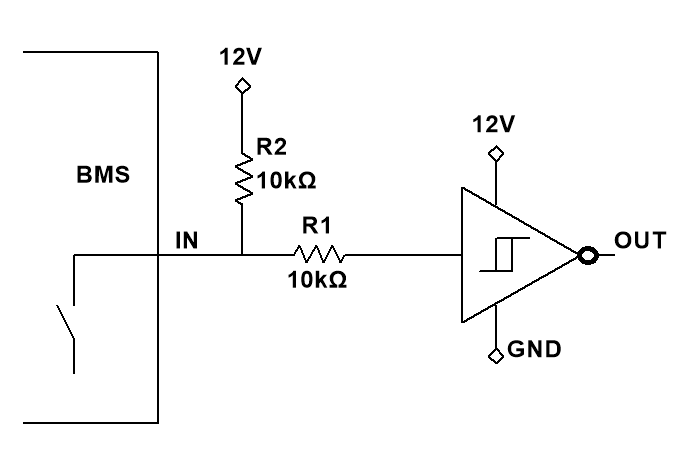
\includegraphics[width=1.00\textwidth]{Inverter.png}
	\caption{Die Inverterschaltung, welche sechs mal verwendet wurde}
	\label{fig:Inverter}
\end{figure}
\color{black}

\paragraph{Blau: Ladezustand}
Da beide Batterien von unabhängigen Batteriemanagementsystemen überwacht werden, können sie auch einen unterschiedlichen Ladezustand aufweisen. Es ist deswegen zweckmässig, den jeweils tieferen Ladestand anzeigen zu lassen, um damit den schlechtesten Fall abzudecken. Diese Signale werden vom BMS in Form eines $5$ kHz PWM-Signales zur Verfügung gestellt. Die Idee des Herstellers ist, dass dieses Signal direkt auf ein analoges Messgerät eingespeist wird, dessen Massenträgheit das Signal glättet. Da beim Detroit lediglich ein Anzeigegerät zur Verfügung steht, müssen diese Signale bereits vorzeitig verglichen werden.

Aus diesem Grund werden die beiden Signale zuerst durch ein eingangsseitiges Tiefpassfilter geglättet. Die Operationsverstärkerstufe $U_{7A}$ vergleicht anschliessend die beiden Signale und gibt ein Signal 0 oder 1 aus, je nachdem, nach welchem Tiefpass eine höhere Spannung anliegt. Um unnötige Schaltvorgänge bei beinahe gleichen Signalen zu verhindern, ist mit Hilfe der beiden Widerstände $R_{19}$ und $R_{20}$ eine Hysterese eingebaut.

Der Transistor $Q_1$ kann mit dem Signal von $U_{7A}$ direkt angesteuert werden. Da jedoch im umgekehrten Fall ebenfalls ein MOSFET verwendet werden soll, muss dieses Signal invertiert werden. Zu diesem Zweck vergleicht der Operationsverstärker $U_{7B}$ dieses Signal mit der halben Versorgungsspannung, wobei das Signal 1 deutlich über dieser liegt, das Signal 0 deutlich darunter. Dieses invertierte Signal wird an das Gate des Transistors $Q_2$ angelegt.

Es steht nun eine Spannung zur Verfügung, welche dem jeweils tieferen der beiden geglätteten PWM-Signalen entspricht. Da das verwendete Voltmeter jedoch verhältnismässig niederohmig ist, wird mit dem Operationsverstärker $U_{7C}$ und dem MOSFET $Q_9$ eine Spannungsfolgerschaltung gebildet. Der Operationsverstärker vergleicht dabei sein Eingangssignal mit der Spannung, welche am Ausgang des Spannungsfolgers anliegt.

Auch bei dieser Schaltung müssen die MOSFETs nur vergleichsweise langsam schalten. Aus diesem Grund wurde für deren Anschluss die selbe Schaltung wie bei den Treiberstufen gewählt. Lediglich beim Spannungsfolger wurde davon abgewichen. Da der Spannungsteiler der beiden Widerstände $R_{27}$ und $R_{28}$ die Spannung nicht verfälschen soll, ist der Gateanschluss über das Voltmeter mit Masse verbunden. Die Idee dahinter ist, dass bei ausgeschaltetem Eingangssignal der Innenwiderstand des Messgerätes im Vergleich zu $R_{28}$ klein ist, also sowieso nicht ins Gewicht fällt. Bei Funktion der Schaltung existiert der Spannungsteiler aber praktisch nicht, da über dem Widerstand lediglich eine sehr kleine Spannung anliegt.
\subsection{Beleuchtung}




\newpage
\section{Steuerung}
In diesem Kapitel werden die einzelnen Schaltvorgänge und -zustände des Fahrzeuges analysiert und beschrieben. Dabei wird besonders auf das Zusammenspiel von mechanisch zu elektrisch eingegangen, aber auch rein mechanische Vorgänge sollen vorgestellt werden.

\subsection{Gashebel}
Die wohl direkteste Verbindung von mechanischer und elektrischer Steuerung geschieht mit dem Gashebel. Dieser kennt dabei mechanisch mehrere Zustände, die die benötigten elektrischen Schaltungen herstellen.

\paragraph{Parken}
Im Zustand Parken ist der Detroit durch die Handbremse gesichert. Diese blockiert die Hinterräder und unterbricht gleichzeitig den Hauptstromkreis durch den Cut-Out-Switch. Gleichzeitig zeigt der Ganghebel in der neutralen Position vertikal nach oben, womit der Rear-Reverse-Switch ebenfalls keinen Kontakt macht. Somit ist Hauptstromkreis sogar zweifach unterbrochen.

\paragraph{Parken zu Neutral}
Im Zustand Neutral ist der Oldtimer nicht mehr durch die Handbremse gesichert. Um diese zu lösen sind zwei Schritte gleichzeitig notwendig. Zum einen soll der Ganghebel in waagerechte Position gebracht werden um ihn dann anschliessend zu sich zu ziehen. Das ist sogleich die Motorbremse, welche die eigentliche Bremsung bei Bedarf unterstützen kann. Damit wird der Sicherungshebel des Cut-Out-Switch betätigt. Somit ist es nun möglich mit dem zweiten Schritt die Handbremse zu betätigen, wodurch sich die Handbremse und sogleich der Cut-Out-Switch aus der Verankerung heben lassen um sich zu lösen und den Hauptstromkreis zu schliessen.

\paragraph{Neutral zu Parken}
Durch die Betätigung der Handbremse wird eine Feder über Zahnräder gespannt und der Cut-Out-Switch unterbricht den Stromkreis. Zu beachten ist, dass die Handbremse mit voller Kraft durchgedrückt wird, damit der Stromkreis klar unterbrochen ist.

\paragraph{Neutral zu Vorwärts}
Durch das Stellen des Ganghebels in waagrechte Position wird der Rear-Reverse-Switch in die Position Vorwärts geschaltet. Das Wegdrücken des Ganghebels wird mit einem Einrasten. Dies setzt einen Hebel in Bewegung, welcher bis hin zum Stufenschalter führt. So dreht dieser nun in Position 1 und das Fahrzeug fährt im 1. Gang los. Ist das Anfahren nun geschehen, kann in den 2. Gang geschaltet werden. Dies erfolgt durch weiteres Wegdrücken des Ganghebels, bis dieser wieder einrastet. Höhere Gänge bis zum 5. können mit der selben Methode erreicht werden.

\paragraph{Neutral zu Rückwärts}
Bei einer 45$^\circ$-Stellung des Ganghebels verschiebt sich der Rear-Reverse-Switch in Position Rückwärts, womit der Stromfluss, wie der Name des Switch schon sagt, umkehrt. Durch gewohntes Schalten in den ersten Gang dreht der Stufenschalter wieder in Position 1 und das Fahrzeug lässt sich rückwärts lenken.
\subsection{Bremsen des Detroits}\label{bremse}

In diesem Kapitel werden die verschiedenen Bremstechniken des Detroits behandelt. Zum einen ist das die Trommelbremse, welche die Räder direkt bremst und zum anderen die Motorbremse, die den ganzen Antriebsstrang bremst. Zu guter Letzt wird noch ein Blick auf die elektrische Bremse gerichtet. Diese ist im Detroit nicht verbaut, jedoch sind sie heute normalerweise in modernen Elektrofahrzeugen aufzufinden.

\paragraph{Trommelbremse}

Grundsätzlich ist die Trommelbremse eine Reibungsbremse bei welcher Bremsbeläge auf eine zylindrische Fläche wirken. Diese Art der Bremsung ist veraltet und wird heutzutage durch die Scheibenbremse ersetzt. Durch betätigen der Bremse mit dem Fuss wird ein Hebel in Bewegung versetzt, welcher an den Bremsen der beiden hinteren Rädern bremst. Die normale Bremse kann auch durch die Handbremse arretiert werden. Dabei ist die Feder der Bremse immer angezogen.

\paragraph{Motorbremse}

Die Motorbremse ist sozusagen eine Manöverbremse, die bei kurzen und sanften Bremsungen eingesetzt werden kann. Dabei drücken Bremsbeläge direkt auf den Rotor des Motors, wodurch dieser gebremst wird. Diese kann durch Ziehen am Ganghebel betätigt werden.

\paragraph{Elektrische Bremse}
Bei modernen elektrischen Fahrzeugen wird das Fahrzeug elektrisch gebremst. Dazu wird der Motor als Generator verwendet und die Energie entweder an den Ursprungsort (Netz oder Batterie) zurück gespeist oder über einen Heizwiderstand in Wärme umgewandelt. Dies hat gegenüber herkömmlichen mechanischen Bremsen den Vorteil, dass die Bremse keinen Verschleiss aufweist und auch nicht überhitzen kann.

Das Erzeugen elektrischer Energie ist mit einer Gleichstrommaschine möglich. Zu diesem Zweck muss die induzierte Spannung (siehe Kapitel \ref{gm} im Anker grösser werden als die Spannung, welche an den Klemmen angelegt wird, also beispielsweise die Batteriespannung. Ist dies der Fall, kehrt sich die Flussrichtung des Stromes um, wodurch die Maschine Energie liefert und als Generator arbeitet.

Mit dem Motor des Detroits könnte diese Funktion rein theoretisch ausgeführt werden, es ist jedoch aus mehreren Gründen nicht praxistauglich. Die Schaltung des Stufenschalters schaltet den Motor in jedem Fall als Reihenschlussmotor. Wird bei dieser Motorverschaltung von aussen Moment zugeführt, so beschleunigt sich lediglich der Anker und es wird weniger Strom für den Antrieb benötigt. Durch den geringeren Stromfluss sinkt jedoch auch die Erregung und mit ihm die induzierte Spannung, es wird also wieder ein neues Gleichgewicht hergestellt.

Rein theoretisch betrachtet wäre es jedoch möglich, mit einer anderen Verschaltung des Stufenschalters ebenfalls eine fremderregte Maschine zu verschalten. Dadurch wäre es möglich, dass die induzierte Spannung des Ankers grösser wird als die Klemmenspannung der Batterien und sich dadurch die Stromrichtung umdreht, ohne dabei das Erregerfeld zu beeinflussen. Um damit aber den Strom, und damit das Bremsmoment, halbwegs konstant zu halten wäre es nötig, entweder die Erregung oder die Klemmenspannung des Motors feinstufig regeln zu können. Dies würde einerseits eine saubere Regelung, andererseits auch zumindest im Falle der Klemmenspannung einen Stromrichter erfordern. Vermutlich wäre jedoch auch ein zweiter Stromrichter nötig gewesen, um die hohen Ströme bei niedriger Spannung für die Erregerwicklungen herzustellen.

Wird ausserdem betrachtet, dass die Leistung des Fahrzeugs sowieso nicht für steile Bergfahrten gereicht hätte, bei denen bei der Abfahrt (auch aufgrund der damals schlechteren Strassen) wirklich stark gebremst worden wäre und auch die maximal erreichbare Geschwindigkeit ebenfalls verhältnismässig klein war, kommt man zum Schluss dass die rekuperierbare Energie nicht besonders gross geworden wäre (insbesondere im Vergleich zu heutigen, deutlich leistungsfähigeren Fahrzeugen). Zusammen mit dem grossen Aufwand für die elektrische Bremse hätte dies ein sehr schlechtes Verhältnis von Aufwand zu Nutzen ergeben.
\subsection{Richtungssteuerung}

Die Richtungssteuerung im Detroit funktioniert nicht wie bei einem normalen Fahrzeug. Unterhalb des Ganghebels befindet sich der Richtungshebel. Durch Bewegungen dieses Hebels werden weitere Hebel verwendet um dann die Vorderachse zu steuern. Dieser Hebel lässt sich in waagrechter Position nach vorne und zurück schieben, wobei nach vorne Richtung links und nach hinten Richtung rechts bedeutet. Möchte der Fahrer aussteigen, können beide Hebel nach oben geklappt werden.


\newpage
\section{Das neue Ladegerät}
Um die Batterien zu Laden wurden zwei neue Ladegeräte installiert. Dies hat den Grund, dass die beiden Batterien unabhängig voneinander geladen werden sollen. Dabei wurde ausserdem die Bedingung gestellt, dass das Fahrzeug an einer Steckdose $230$ VAC/$10$ A geladen werden kann. Das reduziert den maximalen Eingangsstrom pro Ladegerät auf $5$ A, sodass man (mit einem optimalen Wirkungsgrad und ohne Blindleistung) die maximale Ladeleistung berechnen kann:
\begin{equation*}
	P_{max}=U\cdot I=5\text{ A}\cdot230\text{ V}=1150\text{ W}
\end{equation*}
Diese Betrachtung gilt jedoch nur für ideale Bauteile. Um diese Bedingung auch mit realen Bauteilen einzuhalten, wurde ein Netzgerät mit einer Ausgangsleistung von $700$ W gewählt, dessen Eingangsstrom bei $220$ VAC maximal $4.5$ A beträgt. So ist bei einer nominalen Spannung von $48$ V ein Ladestrom von $15$ A möglich, was eine Ladezeit von ungefähr 12 Stunden für eine Komplettladung ermöglichen sollte \cite{ladegeraet}.

\paragraph{Ladeverfahren}
Das Ladegerät lädt die Batterien mit dem sogenannten "\textbf{C}onstant \textbf{C}urrent/\textbf{C}onstant \textbf{V}oltage (CCCV)" Verfahren. Der Ladevorgang kann so grob in zwei Phasen unterteilt werden:

In der ersten Phase wird die Batterie mit einem \textbf{konstantem Strom} geladen, das Lädegerät fungiert dabei als Stromquelle. Durch den konstanten Strom wird die maximale Ladeleistung begrenzt, wodurch thermische Überlastungen der Batterie oder des Ladegerätes vermieden werden können. Falls die Batteriespannung zu Beginn sehr tief ist, die Batterie also tiefentladen ist, wird die Ladung mit einem kleineren Strom begonnen. Durch das Laden steigt die Zellspannung der Zellen an, wodurch sich auch die Spannung der Batterie erhöht. Diese Phase wird beendet, wenn die Spannung an der Batterie auf die Ladeschlussspannung angestiegen ist.

In der zweiten Phase wird mit einer \textbf{konstanten Spannung} geladen. Dabei dient das Ladegerät als Spannungsquelle, die Klemmenspannung der Batterie bleibt konstant. Dabei steigt die Ladung der Zellen weiter, wodurch sich der Strom reduziert. Diese Phase wird beibehalten, bis der Strom unter einen definierten Wert fällt. Beim verwendeten Netzgerät ist dies $\frac{1}{6}$ des Nennstromes, also $\frac{1}{6}\cdot 15\text{ A}=2.5\text{ A}$.

Nach Beendigung der zweiten Phase gilt die Batterie als vollgeladen und der Ladezustand wird beendet. Das Ladegerät überwacht nun lediglich die Zellspannung, wobei beim Unterschreiten einer bestimmten Spannung die fehlende Ladung wieder ergänzt wird. Für die Ladekurven sei auf die Bedienungsanleitung des Netzgerätes \cite{ladegeraet} und Abbildung \ref{fig:liion_akku_kurve} verwiesen.

\paragraph{Vorzeitiger Abbruch des Ladevorgangs}
Der Ladevorgang wird durch das Batteriemanagementsystem überwacht. Dieses kann, über ein Relais, die Stromzufuhr zum Ladegerät und damit den Ladevorgang vorzeitig abbrechen. Dies kann aus folgenden Gründen geschehen: \begin{itemize}
	\item Die Spannung einer Einzelzelle überschreitet die maximale Zellspannung
	\item Die Temperatur einer Zelle überschreitet die Maximaltemperatur
	\item Der Ladestrom überschreitet den maximalen Zellenstrom, dies deutet auf einen Defekt des Ladegerätes hin
	\item Es wird trotz aktivem Ladegerät kein Ladestrom vom BMS gemessen
	\item Defekt an einer Einzelzelle
\end{itemize}
Das BMS überwacht die Batterien auch nach dem Ausschalten des Ladegerätes und kann so, beispielsweise nach dem Abkühlen der Zellen, den Ladevorgang wieder starten.

\paragraph{Balanciervorgang}
Aufgrund minimaler Unterschiede der Einzelzellen ist es möglich, dass sich die Zellen ungleichmässig laden. Bei den parallel geschalteten Zellen kann dies nicht passieren, da diese durch die Parallelverdrahtung auf dem selben Potential gehalten werden. Bei den Seriellverdrahteten Zellen ist dies jedoch sehr gut möglich.

Auf den Modulen des Batteriemanagementsystems befinden sich deswegen sogenannte Balancierwiderstände. Dies sind Widerstände, die Einzelzellen entladen können, um so die Spannung der Einzelzellen auszugleichen. Diese werden vom Batteriemanagementsystem angesteuert und arbeiten in zwei Phasen. In der ersten Phase wird bereits vor dem Ende des Ladeverfahrens die Ladung der Zellen mit einer höheren Spannung verringert, nach Abschluss der Ladung werden alle Zellen an die geringste Zellspannung angepasst. Im Normalbetrieb, wenn sich die Zellen nur minimal unterscheiden, sollten diese Ausgleichsvorgänge aber sehr minim sein. Es wird dadurch vor allem ein Aufschaukeln dieses Effektes vorgebeugt.
\clearpage{\pagestyle{empty}\cleardoublepage}

\chapter{Schlusswort}
\clearpage{\pagestyle{empty}\cleardoublepage}

%%%%%%%%%%%%%%%%%%%%%%%%%%%%%%%%%%%%%%%%%%%%%%%%%%%%%%%%%%%%%%%%%%%%%%%%%%%%%%%%
% Abbildungsverzeichnis
%%%%%%%%%%%%%%%%%%%%%%%%%%%%%%%%%%%%%%%%%%%%%%%%%%%%%%%%%%%%%%%%%%%%%%%%%%%%%%%%
%\clearpage{\pagestyle{empty}\cleardoublepage}
%\listoffigures %Abbildungsverzeichnis
%\clearpage{\pagestyle{empty}\cleardoublepage}

\label{lastBericht}
%%%%%%%%%%%%%%%%%%%%%%%%%%%%%%%%%%%%%%%%%%%%%%%%%%%%%%%%%%%%%%%%%%%%%%%%%%%%%%%%
% Anhang
%%%%%%%%%%%%%%%%%%%%%%%%%%%%%%%%%%%%%%%%%%%%%%%%%%%%%%%%%%%%%%%%%%%%%%%%%%%%%%%%
%\clearpage{\pagestyle{empty}\cleardoublepage}
%\addtocontents{toc}{\protect\setcounter{tocdepth}{-1}}
\appendix
\clearpage{\pagestyle{empty}\cleardoublepage}
\bibliographystyle{IEEEtran}
\bibliography{Bibliographie}
%\pagenumbering{Roman}
%\fancypagestyle{plain}{\fancyhf{}
  %\renewcommand\headrulewidth{0pt}\fancyfoot[C]{\thepage\ / \pageref{LastPage}}}
\pagestyle{plain}

\newpage



% Aufgabenstellung
%%%%%%%%%%%%%%%%%%%%%%%%%%%%%%%%%%%%%%%%%%%%%%%%%%%%%%%%%%%%%%%%%%%

%\begin{figure}[h!]
%\begin{center}
%	\includepdf[pages=-]{images/attachement/%Lastenheft_EIT_P4_16FS.pdf}
	
%\end{center}
%\end{figure}
%\end{appendices}
%\clearpage{\pagestyle{empty}\cleardoublepage}

\end{document}
